\subsection{Dissecting Outbound Delay} 
\label{s:outbound_meas}

%We define the egress delay as the difference between the time when the switch
%issues the flow\_mod and/or packet\_out message and the time when the first
%packet of a particular flow is sent out by the switch. 
% We used the customized controller interfaces to control the \flowmod\ message
% generation. 
%by controlling the matching fields and priorities of the \flowmod\ messages. 

We now study the outbound latencies for three different \flowmod\
operations: insertion, modification, and deletion. For each operation, we
examine the latency impact of key factors, including table
occupancy and rule priority.

Before measuring outbound latency, we install a single default low priority
rule which instructs the switch to drop all traffic. We then install a set of
non-overlapping OpenFlow rules that
%that each specify a destination IP address (other fields are
%wildcarded); we show in \secref{s:meas_insert} that the number of match
%fields specified does not impact rule insertion latencies.  All rules
%instruct the switch to
output traffic on the port connected to the
eth2 interface of our measurement host. For some experiments, we 
systematically vary the rule priorities.
%We then install bursts of OpenFlow rules by sending back-to-back \flowmod
%messages from the controller. Each rule matches a unique destination IP
%address (other fields are wilcards), and, in some cases, has a higher or
%lower priority than the preceding rule. 

%Before we perform the outbound delay measurements, first we install a single
%default low priority rule which instructs the switch to drop all the traffic.
%Then we install specially designed Openflow rules at the switch; while
%they simply specify the destination IP address leaving other fields
%wildcarded, they  may have different priorities. All 
%instruct the switch to output traffic to the port which is connected  
%to the measurement host on which we are monitoring.  

% By default, the table
% has only one rule that drops all packets~\footnote. 
%\li{Is the default rule has a lower
%  priority in the same priority experiment? Should we say this does not impact
%  our experiemental results? }


%\marina{give an example of what we mean increasing rule priority and decreasing
%  rule priority}. 
%Our egress delay measurements make a distinction between the
%flow\_mod and pkt\_out events.  
%By contrast previous measurement work \ref{maple, ucsdHiFi13} for egress delay, only
%captured the "packet out" delay. Thus our approach helps provide a more detailed
%analysis of the egress delay.  

% The priority of a rule indicates its position in the TCAM. Inserting a higher priority
% rule can displace many lower priority rules. To investigate how priority rule
% affects outbound delay. We perform a burst of $n$ \flowmod\ operations with the
% same, increasing, decreasing priority respectively. The \flowmod\ operations are
% insertion, modification and deletion. We also vary $n$. 

\subsubsection{Insertion Latency}
\label{s:meas_insert}

\begin{figure*}[!tb]
\centering
\subfloat[burst size 100, same priority\label{fig:bcm_burst_100_same_pri}]
  {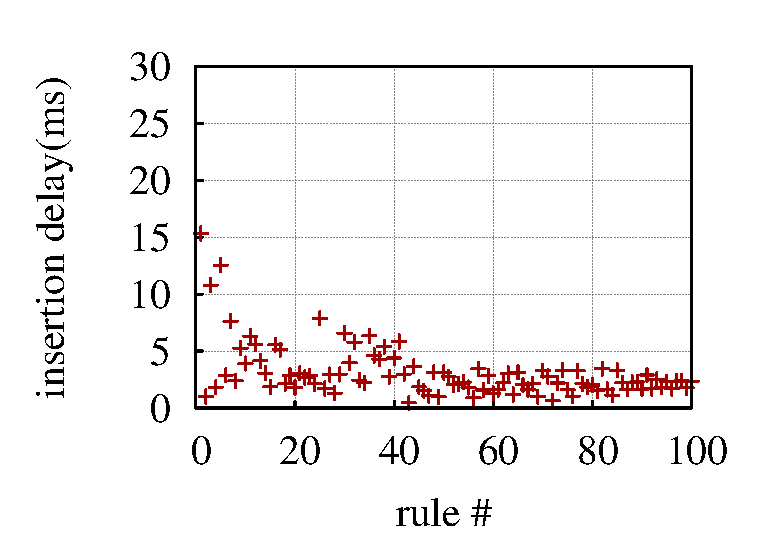
\includegraphics[width=.24\linewidth]{./figs/jan27_bcm_add_same_burst_100.eps}}\hfill
\subfloat[burst size 200, same priority\label{fig:bcm_burst_200_same_pri}]
  {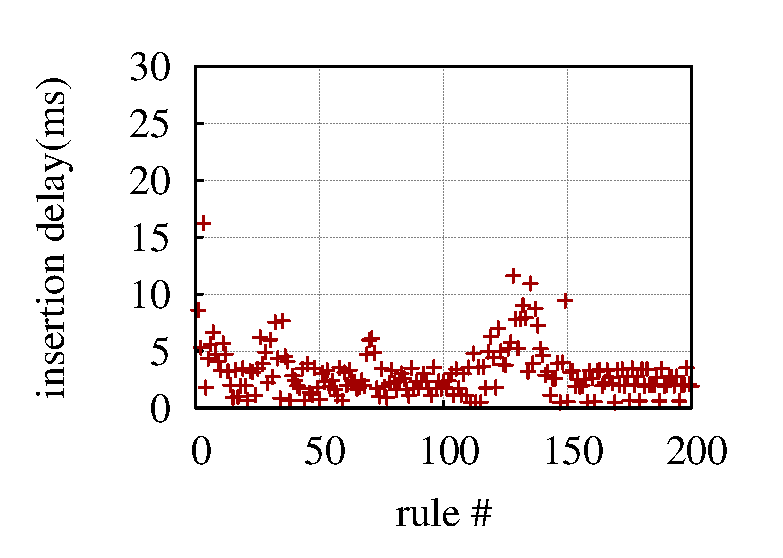
\includegraphics[width=.24\linewidth]{./figs/jan27_bcm_add_same_burst_200.eps}}\hfill
\subfloat[burst size 100, incr. priority\label{fig:bcm_burst_100_incr_pri}]
  {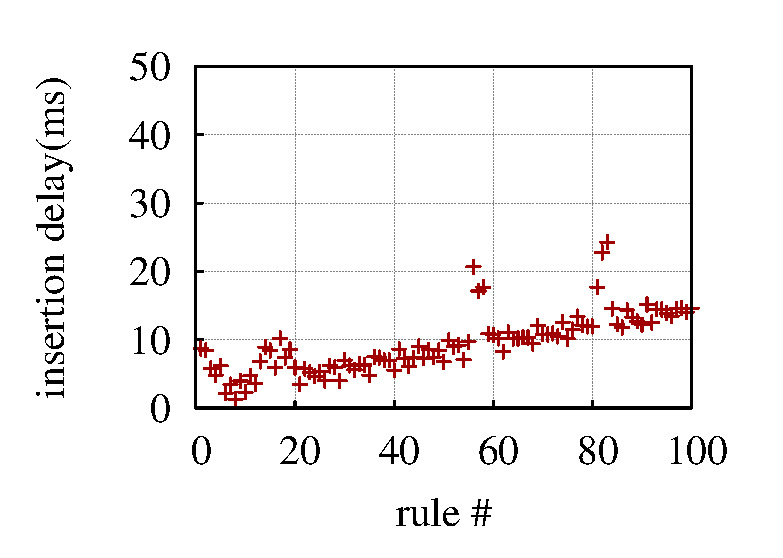
\includegraphics[width=.24\linewidth]{./figs/jan27_bcm_add_incr_burst_100.eps}}\hfill
\subfloat[burst size 200, incr. priority\label{fig:bcm_burst_200_incr_pri}]
  {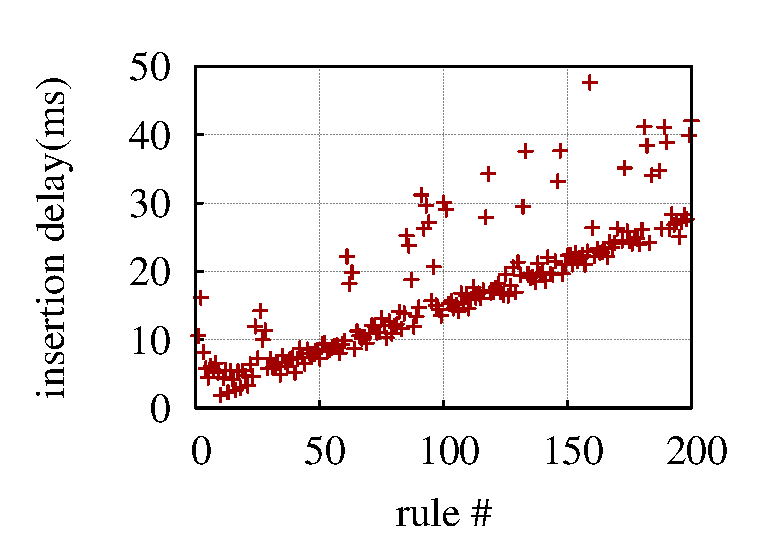
\includegraphics[width=.24\linewidth]{./figs/jan27_bcm_add_incr_burst_200.eps}}
\compactcaption{{\bf \BroadcomOne} priority per-rule {\bf insert} latency}
\label{fig:priority-broadcom-insert}
\end{figure*}


We first examine how different rule workloads impact insertion latency. We
insert a burst of $B$ rules: $r_1,\cdots,r_B$. Let $T(r_i)$ be the time we
observe the first packet matching $r_i$ emerging from the output port
specified in the rule. We define per-rule insertion latency as $T(r_i)-T(r_{i-1})$.  

%We conduct a variety of tests to examine how different patterns of
%rule workloads impact insertion latency. In almost all experiments, we
%install a burst of rules. Let us denote these rules
%in a sequence as $r_1, r_2,\cdots,r_i,\cdots, r_B$. Denote $T(r_i)$ as the time we
%observe the first packet matching $r_i$ emerging from the intended port of the rule
%action. We define insertion latency as $T(r_i)-T(r_i-1)$.  

\minisection{Rule Complexity} 
To understand the impact of rule complexity (i.e., the number of header 
fields specified in a rule), we install bursts of rules that specify either
2, 8, or 12 fields. In particular, we specify destination IP and EtherType
(others wilcarded) in the 2-field case; input port, EtherType, source and
destination IPs, ToS, protocol, and source and destination ports in the
8-field case; and all supported header fields in the 12-field (exact match)
case. We use a burst size of 100 and all rules have the same priority.

We find that rule complexity {\em does not} impact insertion latency. The
mean per-rule insertion delay for 2-field, 8-field, and exact
match cases is 3.31ms, 3.44ms, and 3.26ms, respectively, for \BroadcomOne.
Similarly, the mean per-rule insertion delay for \Intel, \IBM, and
\BroadcomThree is $\approx$ 1 ms irrespective of the number of fields. 
All experiments that follow use rules with 2 fields.

\minisection{Table occupancy} To understand the impact of table occupancy, we
insert a burst of $B$ rules into a switch that already has $S$ rules
installed. All $B+S$ rules have the same priority. We fix $B$ and
vary $S$, ensuring $B+S$ rules can be accommodated in each switch's hardware
table.

We find that flow table occupancy {\em
does not} impact insertion delay if all rules have the same priority.
Taking $B=400$ as an example, the mean per-rule insertion delay is 3.14ms, 
1.09ms, 1.12ms, and 1.11ms (standard deviation 2.14ms, 1.24ms, 1.53ms, and
        0.18ms) for \BroadcomOne, \BroadcomThree, \IBM
and \Intel, respectively, regardless of the value of $S$. 

\minisection{Rule priority} To understand the effect of rule priority on the
insertion operations, we conducted three different experiments each covering
different patterns of priorities. In each, we insert a burst of $B$ rules
into an empty table ($S=0$); we vary $B$. In the {\em same priority}
experiment, all rules have the same priority. In the {\em increasing} and
{\em decreasing priority} experiments, each rule has a different priority and
the rules are inserted in increasing/decreasing priority order, respectively. 

%{\em Same priority.}
Representative results for same priority rules are shown in 
\figsref{fig:bcm_burst_100_same_pri}{fig:bcm_burst_200_same_pri} for
$B=100$ and $B=200$, respectively; the switch is \BroadcomOne. For both
burst sizes, the per-rule insertion delay is similar, with medians of 3.12ms
and 3.02ms, and standard deviations of 1.70ms and 2.60ms for $B=100$ and
$B=200$, respectively. The same priority insertion delays on \BroadcomThree,
\IBM, and \Intel are slightly lower, but still similar: mean per-rule
insertion delay is 1.09ms, 1.1ms, and 1.17ms, respectively, for $B=100$.  We
conclude that {\em same priority} rule insertion delay does not vary with burst
size.

%{\em Increasing priority.}
In contrast, the per-rule insertion delay of increasing priority rules 
{\em increases linearly} with the number of rules inserted for \BroadcomOne,
\BroadcomThree, and \IBM.
\figsref{fig:bcm_burst_100_incr_pri}{fig:bcm_burst_200_incr_pri} shows this
effect for $B=100$ and $B=200$, respectively, for \BroadcomOne.  Compared with
the same priority experiment, the average per-rule delay is much larger:
9.47ms (17.66ms) vs. 3.12ms (3.02ms), for $B=100$ (200). The results are
similar for \BroadcomThree and \IBM: the average per-rule insertion delay is
7.75ms (16.81ms) and 10.14ms (18.63) for $B=100$ (200), respectively. 
We also observe the slope of the latency increase is constant---for a given
switch---regardless of $B$.

The increasing latency in \BroadcomOne, \BroadcomThree, and \IBM stems from
the TCAM storing high priority rules at low (preferred) memory addresses. Each
rule inserted in the {\em increasing priority} experiments displaces all prior
rules!

Surprisingly, latency does not increase when increasing priority rules are
inserted in \Intel. As shown in \figref{fig:intel_burst_800_incr_pri}, the
median per-rule insertion delay for \Intel is 1.18ms (standard deviation of
1.08ms), even with $B=800$! Results for other values of $B$ are similar.
This shows that the \Intel TCAM architecture is fundamentally different from
\Broadcom and \IBM. Rules are ordered in \Intel's TCAM such that higher
priority rules do not displace existing low priority rules. 

However, displacement does still occur in \Intel. 
\figref{fig:intel_burst_800_decr_pri} shows per-rule insertion latencies for
for {\em decreasing priority} rules for $B=800$. We see two effects: (1) the
latencies alternate between two modes at any given time, and (2) there is a
step-function effect after every 300 or so rules. 

A likely explanation for the former is bus buffering. Since rule insertion is
part of the switch's control path, it is not really optimized for latency.
The latter effect can be explained as follows: Examining the \Intel switch
architecture, we find that it has 24 slices, $A_1\ldots A_{24}$, and each
slice holds 300 flow entries. There exists a consumption order (low-priority
first) across all slices.  Slice $A_i$ stores the $i^{th}$ lowest
priority rule group. If rules are inserted in decreasing priority, $A_1$ is
consumed first until it becomes full. When the next low priority rule is
inserted, this causes one rule to be displaced from $A_1$ to $A_2$.  This
happens for each of the next 300 rules, after which cascaded displacements
happen: $A_1 \rightarrow A_2 \rightarrow A_3$, and so on. We confirmed this
with \Intel.

We observe different trends when inserting {\em decreasing priority} rules
in \BroadcomOne, \BroadcomThree, and \Intel. With \BroadcomOne, we find the
average per-rule insertion delay increases with burst size: 8.19ms for $B=100$
vs. 15.5ms for $B=200$. Furthermore, we observe that the burst of $B$ rules is
divided into several groups, and each group is reordered and inserted in the
TCAM in order of increasing priority. This indicates that \BroadcomOne
firmware reorders the rules and prefers increasing priority insertion.  In
contrast, \BroadcomThree's per-rule insertion delay for decreasing priority
rules is similar to same priority rule insertion: $\approx$ 1ms. Hence, the
\BroadcomThree firmware has been better optimized to handle decreasing
priority rule insertions. The same applies to \Intel: per-rule insertion delay
for decreasing priority rules is similar to same priority rule insertion:
$\approx$ 1.1ms.

%\emph{\BroadcomOne, same priority.} 
%Representative results for $B=100$ and $B=200$ are shown in
%\figsref{fig:bcm_burst_100_same_pri}{fig:bcm_burst_200_same_pri},
%respectively. In both cases, we see that the per-rule insertion delay is
%similar: with medians of 3.12ms and 3.02ms, and standard deviations of 1.70ms
%and 2.60ms, for $B=100$ and $B=200$, respectively.  We conclude that same
%priority rule insertion delay does not vary with burst size on \BroadcomOne.

%\emph{\BroadcomOne, increasing priority.}
%\figref{fig:bcm_burst_100_incr_pri} shows the result for $B=100$. We note that
%the per-rule insertion delay actually {\em increases linearly} with the number
%of rules inserted. \figref{fig:bcm_burst_200_incr_pri} shows the result for
%$B=200$; we see that the slope stays the same as $B=100$.  Compared with the
%same priority experiment, the average per-rule delay is much larger: 9.47ms
%(17.66ms) vs 3.12ms (3.02ms), for $B=100$ (200).  Results for other values of
%$B$ are qualitatively similar.  The TCAM in this switch stores high priority
%rules at low (preferred) memory addresses. Thus, each rule inserted in this
%experiment displaces all prior rules!

%\emph{\BroadcomOne, decreasing priority.} 
%We also perform decreasing priority insertion (not shown). The average
%per-rule insertion delays for $B=100$ and $B=200$ are 8.19ms and 15.5ms,
%respectively. We observe that the burst of $B$ rules is divided into a number
%of groups, and each group is reordered and inserted in the TCAM in order of
%increasing priority.  This indicates that \BroadcomOne firmware reorders the
%rules and prefers increasing priority insertion. 

%\emph{\BroadcomThree, same priority.} 
%The mean per-rule insertion delay is 1.09ms (1.08ms) for $B=100$ (200). Thus,
%similar to \BroadcomOne, the rule insertion time does not vary with burst
%size when all rules are of the same priority. 

%\emph{\BroadcomThree, increasing priority.} 
%The average per-rule insertion delay is much larger: 7.75ms (16.81ms) for $B =
%100$ (200). This is similar to our findings for \BroadcomOne, affirming that
%TCAM organization requirements, not software implementation issues, are the
%primary cause.

%\emph{\BroadcomThree, decreasing priority.} 
%The per-rule delay is similar to that of same priority insertion: $\approx
%1$ms. This contrasts with \BroadcomOne, where decreasing priority insertion
%increases with the number of rules inserted---average of 8.19ms (15.5ms) for
%$B=100$ (200).  Hence the \BroadcomThree firmware has been better optimized to
%handle decreasing priority rule insertions.

%\emph{\IBM, same priority.}
%The \IBM switch's same priority rule insertion performance trend is quite
%similar to that of \Broadcom. When all the inserted rules have the same
%priority, the per-rule insertion latency is around 1.1ms.

%\emph{\IBM,  increasing priority.}
%When it comes to increasing priority, the per-rule insertion latency becomes
%significantly larger.  The average per-rule insertion delays for $B=100$ and
%$B=200$ are 10.14ms and 18.63ms, respectively. 

%\emph{\IBM,  decreasing priority.}
%\IBM switch's per-rule insertion latency in decreasing priority is similar to
%that of same priority rule insertion, namely, around 1.1ms per insertion.

\begin{figure}[!tb]
\centering
\subfloat[burst size 800, incr. priority\label{fig:intel_burst_800_incr_pri}]
  {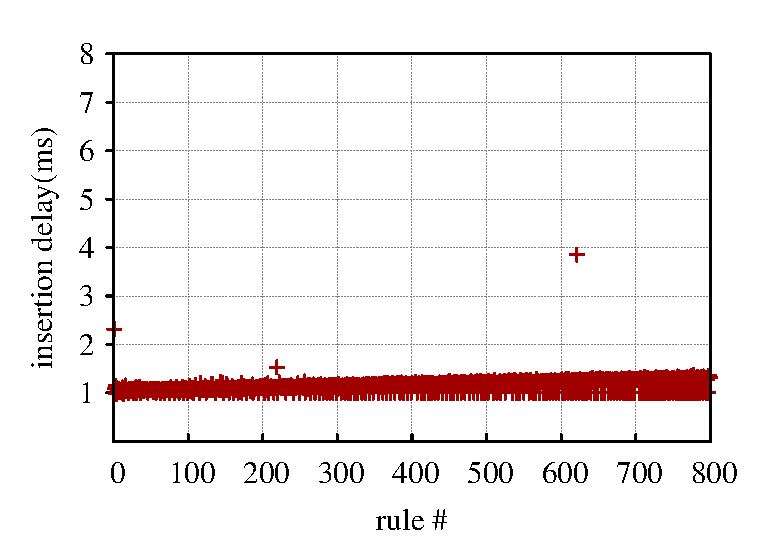
\includegraphics[width=.49\linewidth]{./figs/jan27_intel_incr_burst_800.eps}}\hfill
\subfloat[burst size 800, decr. priority\label{fig:intel_burst_800_decr_pri}]
 {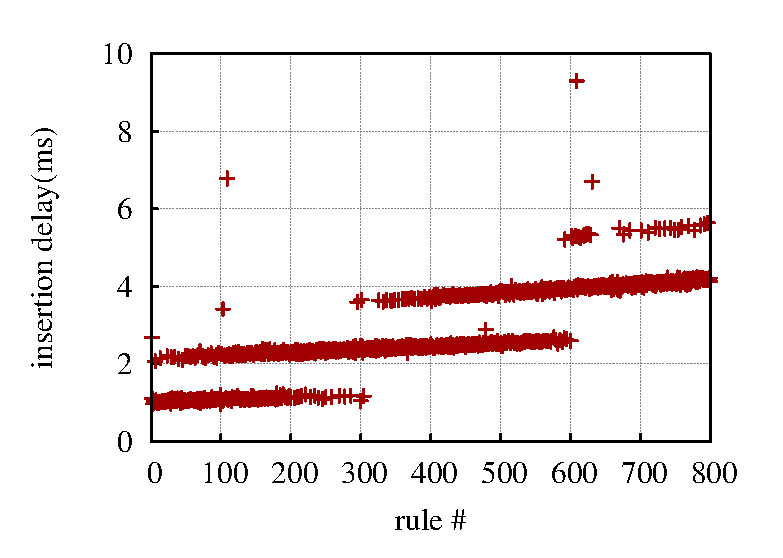
\includegraphics[width=.49\linewidth]{figs/jan27_intel_empty_800L_decr_delta.eps}}
\compactcaption{{\bf Intel} priority per-rule {\bf insert}
} 
\label{fig:priority-intel-insert}
\end{figure}

%\emph{\Intel, same priority.} 
%For $B=800$ on \Intel\footnote{We present results for a larger value of $B$
%because the flow table size on \Intel is larger (\tabref{switch_para}).} we
%see that the per-rule insertion delay is similar across the 800 rules, with a
%median of 1.17ms and standard deviation of 0.16ms (not shown).  The results
%for other values of $B$ are similar. Thus, similar to \BroadcomOne,
%\BroadcomThree, and \IBM same priority rule insertion delay does not vary
%with burst size on \Intel. 

%\emph{\Intel, increasing priority.}
%\figref{fig:intel_burst_800_incr_pri} shows per-rule latencies for $B=800$.
%\emph{Surprisingly}, in contrast with \BroadcomOne, \BroadcomThree, and \IBM,
%the per rule insertion delay among the rules is more or less the same, with a
%median of 1.18ms and a standard deviation of 1.08ms.  We see similar results
%for other values of $B$. This shows that the \Intel TCAM architecture is
%fundamentally different from \Broadcom.  Rules are ordered in \Intel's TCAM
%such that higher priority rule insertion does not displace existing low
%priority rules. 

%\emph{\Intel, decreasing priority.} 
%\figref{fig:intel_burst_800_decr_pri} shows per-rule insertion latencies for
%$B=800$. We see two effects: (1) the latencies alternate between two modes at
%any given time, and (2) a step-function effect after every 300 or so rules. 
%
%A likely explanation for the former is bus buffering. Since rule insertion is
%part  of the switch's control path, it is not really optimized for latency.
%The latter effect can be explained as follows: Examining the \Intel switch
%architecture, we find that it has 24 slices, $A_1\ldots A_{24}$, and each
%slice holds 300 flow entries. There exists a consumption order (low-priority
%first) across all slices.  Slice $A_i$ stores the $i^{th}$ lowest priority
%rule group. If rules are inserted in decreasing priority, $A_1$ is consumed
%first until it becomes full. When the next low priority rule is inserted, this
%causes one rule to be displaced from $A_1$ to $A_2$.  This happens for each of
%the next 300 rules, after which cascaded displacements happen: $A_1
%\rightarrow A_2 \rightarrow A_3$, and so on. We confirmed this with \Intel.


\minisection{Priority and table occupancy combined effects} 
%Given our understanding of the impact of rule priority and table occupancy on
%per-rule insertion latency, we now study their combined impact. 
We now study the combined impact of rule priority and table occupancy.
We conduct two experiments: For the first experiment, the table starts with
$S$ high priority rules, and we insert $B$ low priority rules.  For the
second experiment, the priorities are inverted.
For both experiments, we measure the total time to install all rules in the
burst, $T(r_B)-T(r_1)$.
%burst rule insertion completion time;
%many applications depend on this the metric (\secref{s:apps}). 

\begin{figure}
\subfloat[insert low priority rules into\newline a table with high priority rules\label{fig:bcm_outbound_two_pri_high_low_burstB}]
  {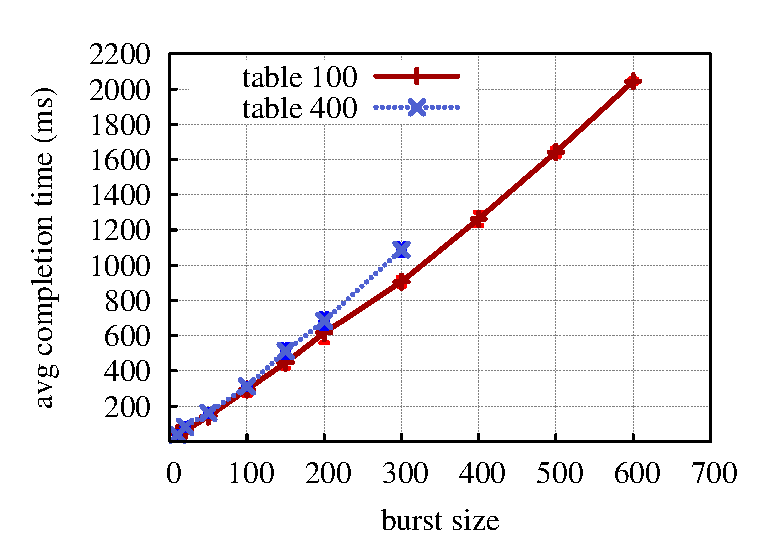
\includegraphics[width=.50\linewidth]{./figs/bcm_two_pri_high_low_burstB.eps}}\hfill
\subfloat[insert high priority rules into a table with low priority rules\label{fig:bcm_outbound_two_pri_low_high_burstB}]
  {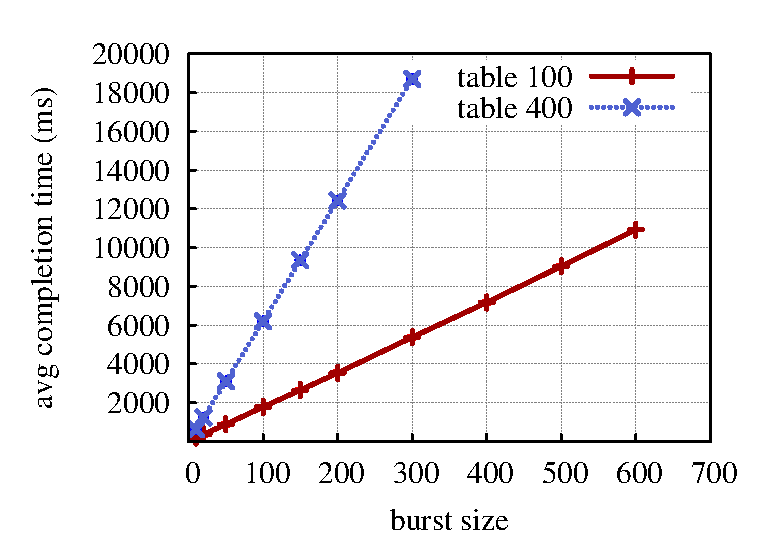
\includegraphics[width=.50\linewidth]{./figs/bcm_two_pri_low_high_burstB.eps}}
\compactcaption{Overall completion time on {\bf \BroadcomOne}.  Initial table occupancy is S high (low) priority rules; insert a burst of low (high) priority rules. Averaged over 5 runs. }
\label{fig:burst-completion-time}
\end{figure}

%We conduct two experiments. With $S$ rules in the table, we insert a burst of $B$ rules. 
%For the first experiment, $S$ has high priority and we insert the burst with low priority. 
%For the second experiment, if it is Broadcom (\BroadcomOne or \BroadcomThree), $S$ has low priority and we insert rules with high priority; if it is Intel, $S$ has high priority and we insert rules in {\em decreasing} priority.

For \BroadcomOne, \BroadcomThree, and \IBM, we expect that as long as the same
number of rules are displaced, the completion time for different values of
$S$ should be the same.
Indeed, from \figref{fig:bcm_outbound_two_pri_high_low_burstB} (for
\BroadcomOne), we see that even with 400 high priority rules in the
table, the insertion delay for the first experiment is no different from the
setting with only 100 high priority rules in the table. In contrast, in
\figref{fig:bcm_outbound_two_pri_low_high_burstB}, newly inserted high
priority rules will displace low priority rules in the table, so when
$S=400$ the completion time is about 3x higher than $S=100$.
%\fixme{added IBM below}
For \IBM (not shown), inserting 300 high priority rules into a table with 400
low priority rules takes more than 20 seconds.  

 
\iffalse
\begin{figure}[!tb]
\centering
\subfloat[decreasing priority\label{fig:intel_burst_100_incr_pri_1}]
  {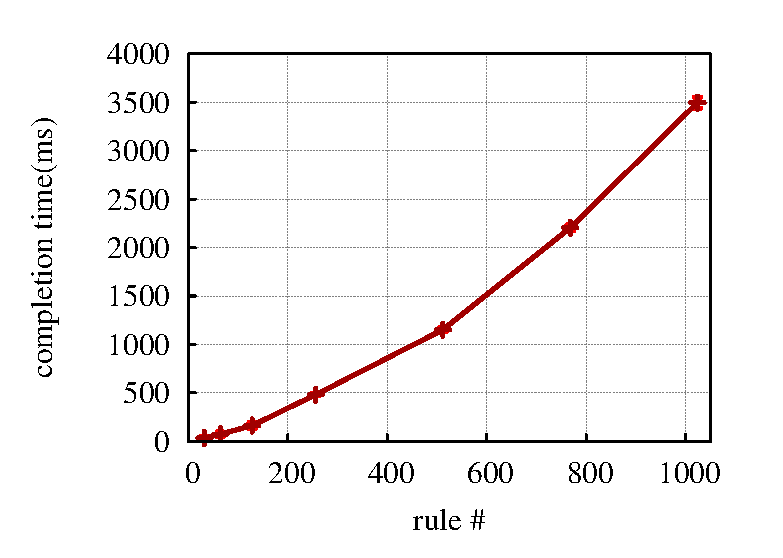
\includegraphics[width=.5\linewidth]{./figs/jan27_intel_decr_burst_size_effect.eps}}\hfill\caption{{\bf Intel} overall completion time} 
\label{fig:priority-intel-insert-more-results}
\end{figure}
\fi

%For \Intel, we also run the same two experiments as for Broadcom. 
For \Intel, the results are similar to same priority rule insertion. This
indicates that \Intel uses different TCAM organization schemes than the
\Broadcom and \IBM switches.  %\fixme{changed}
%optimizes for rule priority better than \BroadcomOne. 
\iffalse
When
we insert in decreasing priority
(\figref{fig:priority-intel-insert-more-results}) the completion time is
about 3.5 seconds, 3x higher than the case of same priority insertion.
\aaron{What is the point of these Intel results?}
\sourav{To show the worst case burst completion time on Intel since it does not have table occupancy effect. But now since the title has been changed from burst completion time to combined effect, I dont think this makes much sense here. }
 \fi
 
\minisection{Summary and root causes}
We observe that: (1) rule complexity does not affect insertion delay; (2)
same priority insertions in \BroadcomOne, \BroadcomThree, \Intel and \IBM are fast
and not affected by flow table occupancy; and (3) priority insertion patterns
can affect insertion delay very differently. For \Intel, increasing priority
insertion is similar to same priority insertion, but decreasing priority 
incurs much higher delay. For \BroadcomThree and \IBM the behavior is inverted:  
decreasing priority insertion is similar to same priority insertion and increasing priority insertion incurs higher delay. For \BroadcomOne, 
insertions with different priority patterns are all much higher than
insertions with same priority. 

Key root causes for observed latencies are: (1) how rules are organized in the TCAM, and (2) the number of slices. {\em Both of these are intrinsically tied to switch hardware.} Even in the best case (\Intel), per-rule insertion latency of 1ms is higher than what native TCAM hardware can support (100M updates/s~\cite{estan:private}). Thus, in addition to the above two causes, there appears to be an {\em intrinsic switch software overhead} contributing to all latencies.

%\aditya{the following is weird} The feedbacks we got from both vendors are that
%their switch firmware has not been 
%optimized for rule priority. 

%\aditya{root causes is incomplete}

\iffalse
Each slice can hold 300 flow entries,
       Also, there exists a consumption order (low-priority first!) across all slices:
       A-slice: the lowest priority rule group, 
       B-slice: the second lowest priority rule group, ….etc  
       In such a case, if the flow rules are inserted in the decreasing priority order,
        A-slice will be first consumed until it becomes full.
        When A-slice is full, B-slice starts to be consumed.
        However, due to the decreasing order, 
       299 existing rules in A-slice must be moved into B-slice
       and then a new inserted rule will be written into A-slice.
       Until B-slice becomes full, and so on.

Based on a phone conversation:
The organization of the TCAM structure is 24 slices x 1024 lines x 36b. There is
also a remap stage between slices 12 and 13. For exact matching 12-tuple
conditions the lookup is split between the 2 halves (pre and post remap stage)
12 slices are used for each of the 12-tuple lookups. Under these conditions then
the OpenFlow table would be limited to 4 groups of 1K entries (4K total). 
If the Key used fewer tuples, or if it could be wild carded the maximum entries
in the TCAM block would be up to 24K. 
There is also an SRAM based Binary Search Tree (longest Prefix match). This is
organized as 4 slices x 16K entries x 32b. If this table is combined with the
TCAM then the maximum flow table size could be as large as 88K entries
(depending on Key size). 
\fi
% LocalWords:  Broadcom TODO Keqiang TCAM feedbacks

\subsubsection{Modification Latency}

We now study  modification operations. As before, we experiment with bursts of rules. Modification latency is defined similar to insertion.

\minisection{\bf Table occupancy} To study the impact of table
occupancy, we pre-insert $S$ rules into a switch,
%(simple rules as before),
all with the same priority. We then modify one rule at a time by changing the
rule's output port, sending modification requests back to back. 

\begin{figure}[!tb]
\centering
\subfloat[100 rules in table \label{fig:bcm_mod_same_burst_100}]
  {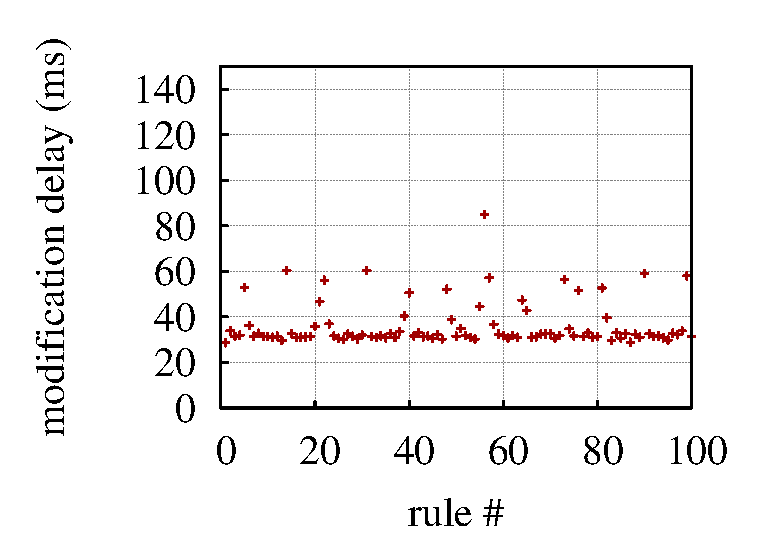
\includegraphics[width=.5\linewidth]{./figs/jan27_bcm_mod_same_burst_100_imc.eps}}\hfill
%\subfloat[burst size 100, increasing priority.\label{fig:bcm_mod_incr_burst_100}]
%  {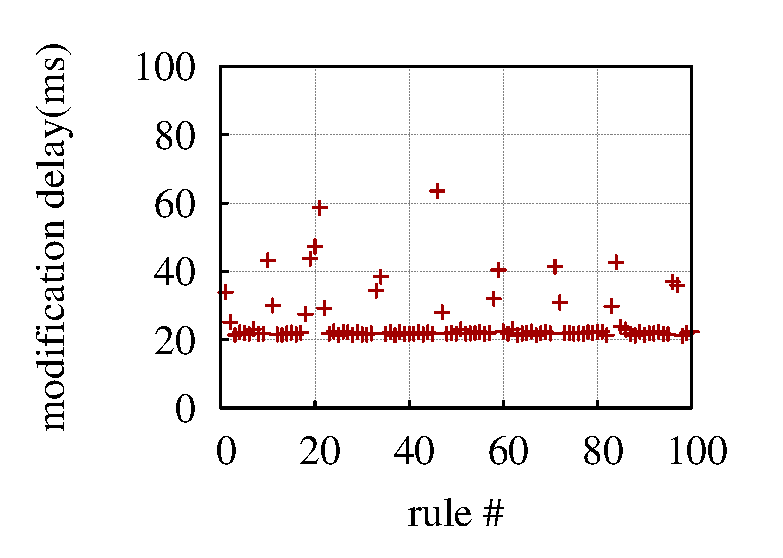
\includegraphics[width=.24\linewidth]{./figs/jan27_bcm_mod_incr_burst_100.eps}}\hfill
%\subfloat[burst size 100, decreasing priority.\label{fig:bcm_mod_decr_burst_100}]
%  {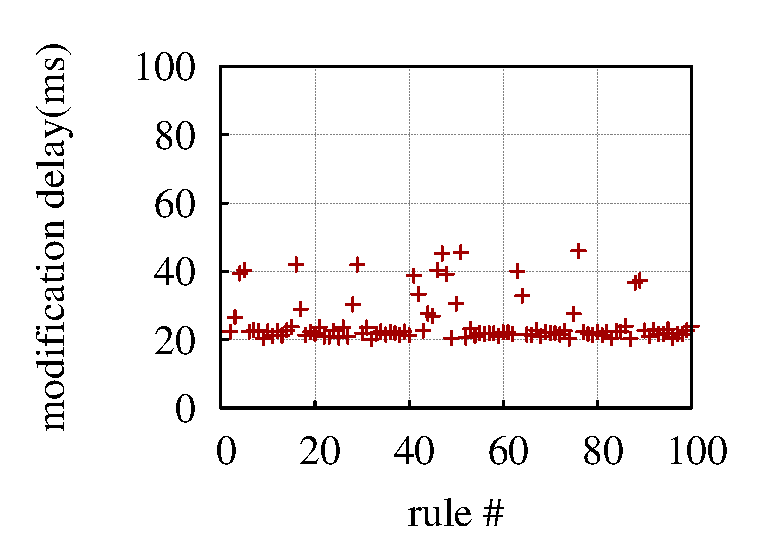
\includegraphics[width=.24\linewidth]{./figs/jan27_bcm_mod_decr_burst_100.eps}}\hfill
\subfloat[200 rules in table \label{fig:bcm_mod_same_burst_200}]
  {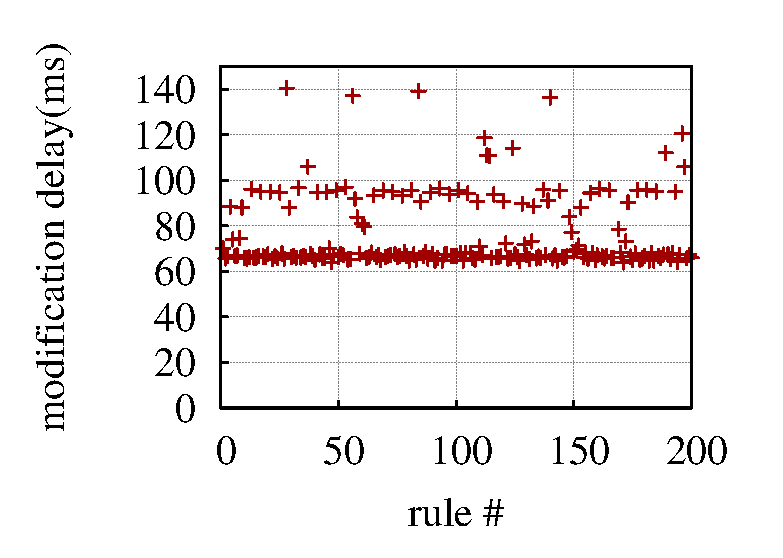
\includegraphics[width=.5\linewidth]{./figs/jan27_bcm_mod_same_burst_200.eps}}
\compactcaption{{\bf \BroadcomOne} per-rule {\bf mod.} latency, same priority}
\label{fig:occupancy-broadcom-modify}
\end{figure}
 
Per-rule modification delay for \BroadcomOne when $S=100$ and $S=200$ are shown in
\figsref{fig:bcm_mod_same_burst_100}{fig:bcm_mod_same_burst_200}, respectively. We
see that the per-rule delay
is more than 30 ms for $S=100$. When we double the number of rules,
$S=200$, latency doubles as well. It grows
linearly with $S$ (not shown). Note that
this latency is much higher than the corresponding
insertion latency (3.12ms per rule) (\S\ref{s:meas_insert}).
%\fixme{IBM added}
\IBM's per-rule modification latency is also affected significantly by the table occupancy---
the per-rule modification latencies for $S=100$ and $S=200$ are 18.77ms and 37.13ms, respectively.
 
\iffalse
\begin{figure}[!tb]
  \centering \subfloat[100 rules in table \label{fig:intel_mod_same_burst_100}]
  {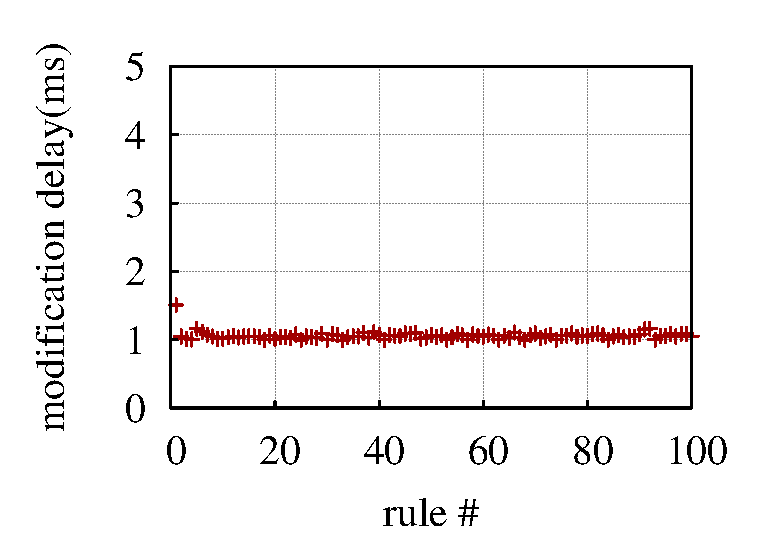
\includegraphics[width=.5\linewidth]{./figs/jan27_intel_mod_same_burst_100.eps}}\hfill
%\subfloat[burst size 100, increasing priority.\label{fig:intel_mod_incr_burst_100}]
%  {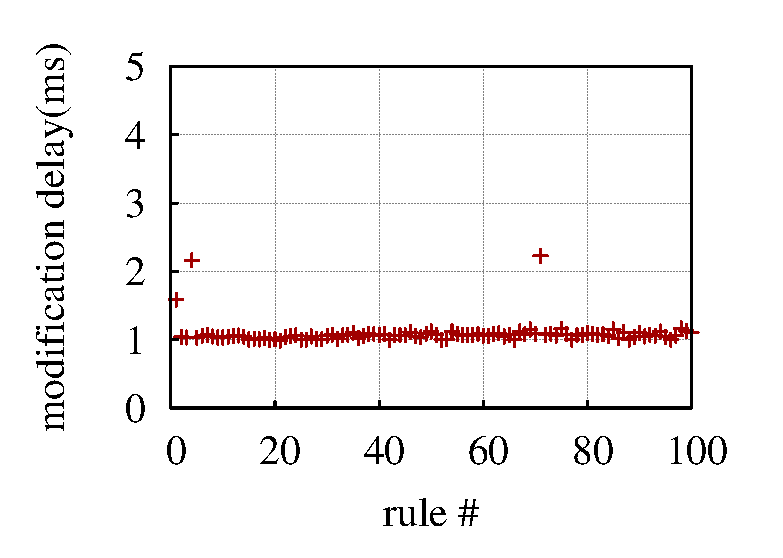
\includegraphics[width=.24\linewidth]{./figs/jan27_intel_mod_incr_burst_100.eps}}\hfill
%\subfloat[burst size 100, decreasing priority.\label{fig:intel_mod_decr_burst_100}]
%  {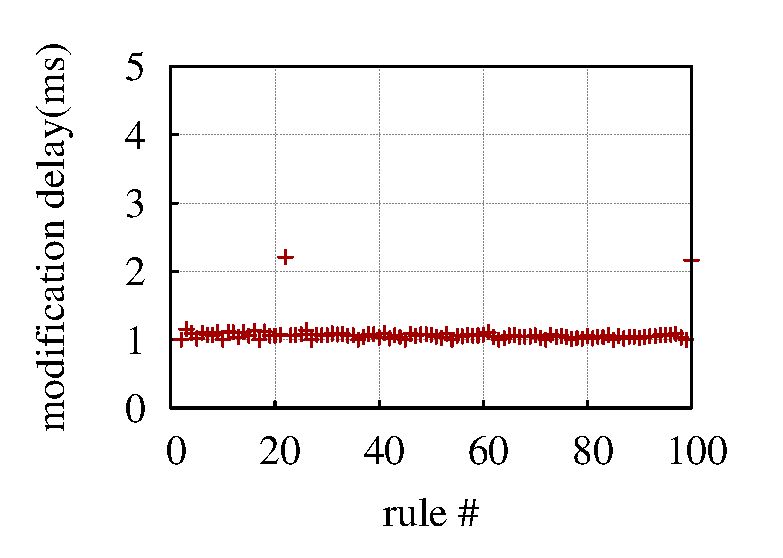
\includegraphics[width=.24\linewidth]{./figs/jan27_intel_mod_decr_burst_100.eps}}\hfill
\subfloat[200 rules in table \label{fig:intel_mod_same_burst_200}]
  {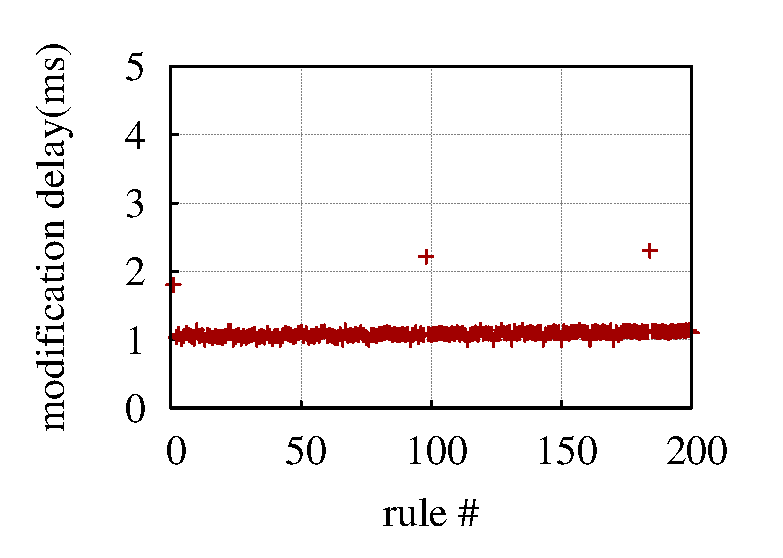
\includegraphics[width=.5\linewidth]{./figs/jan27_intel_mod_same_burst_200.eps}}
\compactcaption{{\bf \Intel} per-rule {\bf mod.} latency, same priority}
\label{fig:occupancy-intel-modify}
\end{figure}
\fi
%The results for $S=100,200$ for Intel are shown in
%Figure~\ref{fig:occupancy-intel-modify}. 
%Sourav commented
%For Intel, the modification delay for $S=100,200$ is around 1 ms
%(standard deviation 0.06) for all modified rules, similar to insertion
%in Figure~\ref{fig:priority-intel-insert}.
%delay with same priority,  in contrast with
%\BroadcomOne. 
% the modification delay is around 1 ms, which is the same as
% the insertion delay when all rules have same priority
% (\S\ref{s:meas_insert}).
% The results are the same for higher values of
% $S$.

In contrast, \Intel and \BroadcomThree  have lower modification delay,
and it does not vary with table occupancy. For \Intel (\BroadcomThree) the
per-rule modification delay for both $S=100$ and $S=200$ is around 1 ms (2ms)
for all modified rules, similar to (2X more than) same priority insertion delay. 

%\aditya{I changed the previous sentences. Check!!}
%%  For \BroadcomThree the average modification delay (standard deviation) for $S=100$ and $S=200$ is 2.19 (1.82) and 2.95 (2.29) respectively.
%For \BroadcomThree the modification delay is highly variable and is 
%related with table occupancy. For example, modifying 200 %rules in a table with 200 and 500 rules takes 449 and %4984 msec respectively. 

\minisection{Rule Priority} We conduct two experiments on each switch to
study the impact of rule priority. In
each experiment, we insert $B$ rules into an empty table ($S = 0$). In the 
{\em increasing} priority experiments, the rules in the table each have a
unique priority, and we send back-to-back modification requests for
rules in increasing priority order. We do the opposite in the {\em
decreasing priority} experiment. We vary $B$.%  across
% experiments. Note that the {\em same priority} experiment here is
% exactly the same as the table occupancy experiment above; hence we
% omit it.

\begin{figure}[!tb]
\centering
%\subfloat[burst size 100, same priority.\label{fig:bcm_mod_same_burst_100}]
%  {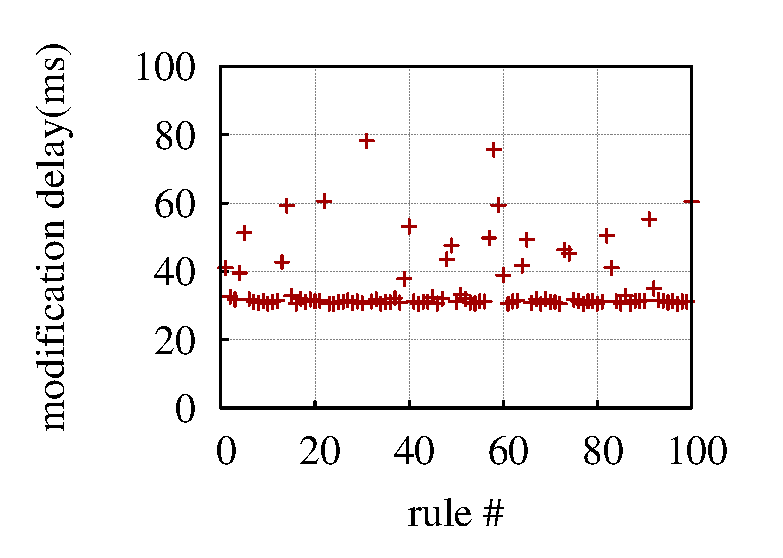
\includegraphics[width=.5\linewidth]{./figs/jan27_bcm_mod_same_burst_100.eps}}\hfill
\subfloat[burst size 100, incr. priority\label{fig:bcm_mod_incr_burst_100}]
  {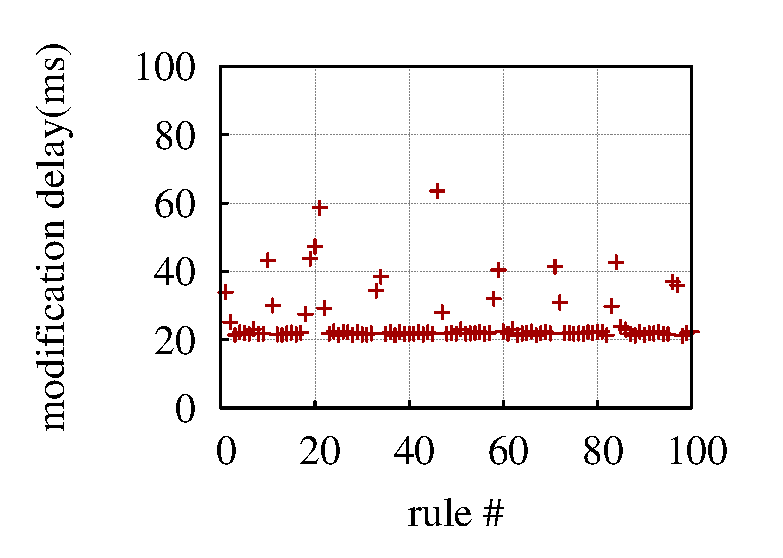
\includegraphics[width=.5\linewidth]{./figs/jan27_bcm_mod_incr_burst_100.eps}}\hfill
\subfloat[burst size 100, decr. priority\label{fig:bcm_mod_decr_burst_100}]
  {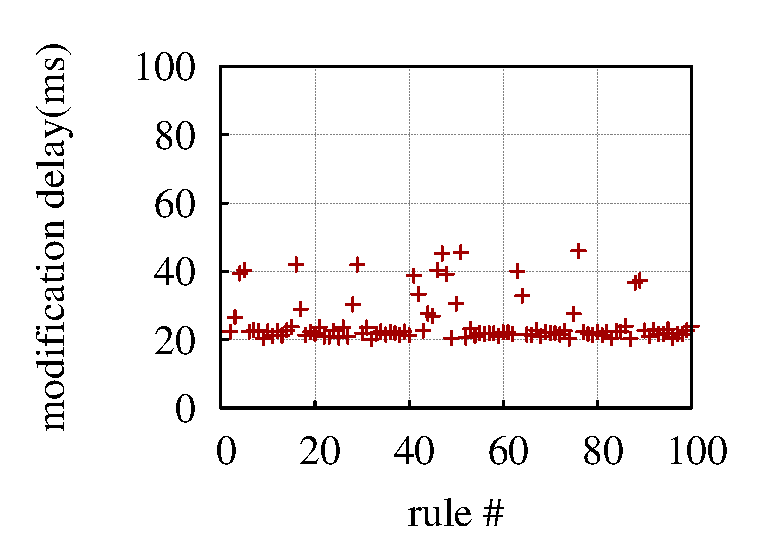
\includegraphics[width=.5\linewidth]{./figs/jan27_bcm_mod_decr_burst_100.eps}}\hfill
%\subfloat[burst size 200, same priority.\label{fig:bcm_mod_same_burst_200}]
%  {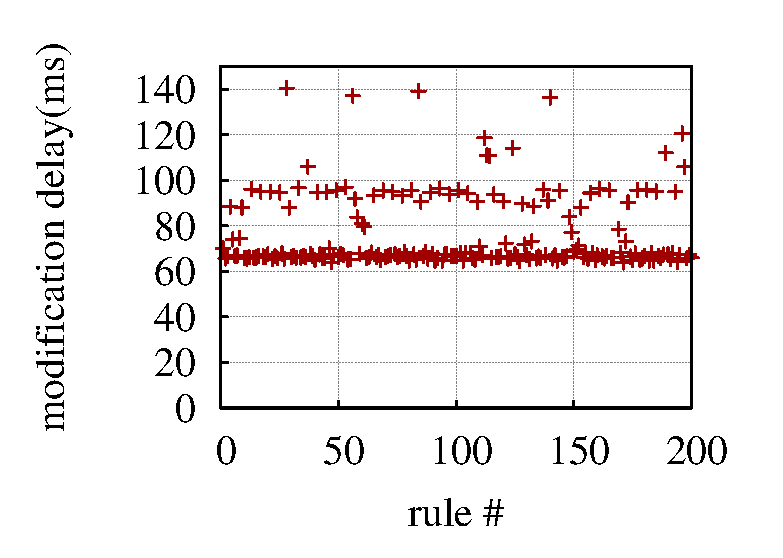
\includegraphics[width=.5\linewidth]{./figs/jan27_bcm_mod_same_burst_200.eps}}
\compactcaption{{\bf \BroadcomOne} priority per-rule {\bf modification} latency}
\label{fig:priority-broadcom-modify}
\end{figure}

%\emph{\BroadcomOne: increasing/decreasing priority.}
\figsref{fig:bcm_mod_incr_burst_100}{fig:bcm_mod_decr_burst_100} show the results for the increasing and decreasing priority experiments, respectively, for
$B=100$ on \BroadcomOne. In both cases, we see: (1) the per-rule modification delay is similar
across the rules, with a median of 25.10ms and a standard deviation of
6.74ms, and (2) the latencies are identical across the experiments. 
We similarly observe that priority does not affect modification delay in
\BroadcomThree, \Intel and \IBM (not shown).
% Again, the
% latencies are  much larger than insertion with same priority, 25 ms vs 3 ms.
%\aditya{this is not true! bcm insertion latencies are also high!} 
%li: add same priority, fixed, right?
%We observed that the latencies grew with $B$ for both experiments.
% increasing and decreasing
% priority experiments.

% Figure~\ref{fig:priority-broadcom-modify}-d shows the results for
% $B=200$, and again the per rule latency is about twice as high as that
% for $B=100$. 
% % per-rule modification delay for 200 rules has a median 60 (xx) ms and
% % standard deviation xx. The modification time is significant impacted
% % by the number of rules in the table.

% \emph{Broadcom: decreasing priority.}  We modify in both increasing rule
%   priority and decreasing rule priority. As shown in
%   Figure~\ref{fig:priority-broadcom-insert}-b,c, the per rule modification delay
%   is not affected by rule priority. Their median delay is xx and xx respectively
%   with standard deviation xx and xx.

%We next describe our measurement results on Intel. 
\iffalse
\begin{figure}[!tb]
\centering
%\subfloat[burst size 100, same priority.\label{fig:intel_mod_same_burst_100}]
%  {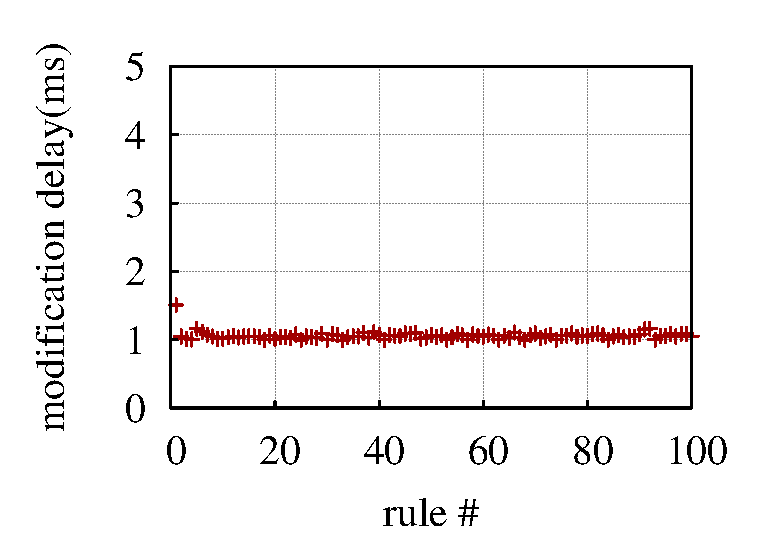
\includegraphics[width=.5\linewidth]{./figs/jan27_intel_mod_same_burst_100.eps}}\hfill
\subfloat[burst size 100, increasing priority.\label{fig:intel_mod_incr_burst_100}]
  {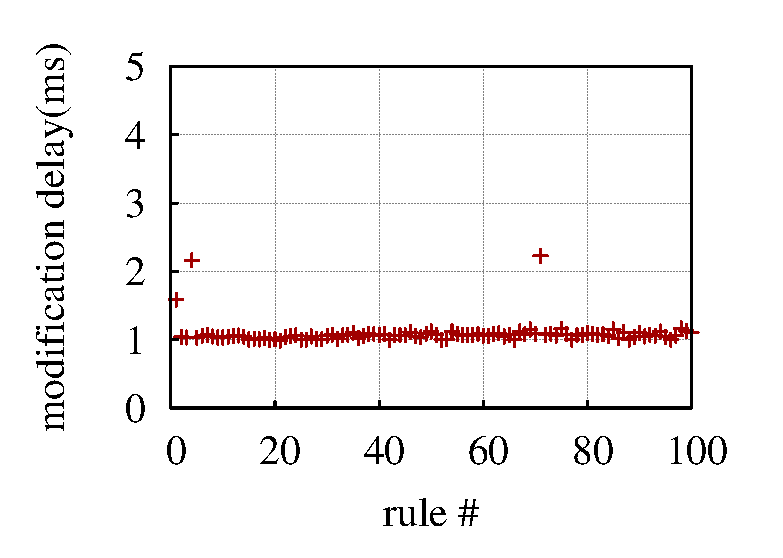
\includegraphics[width=.5\linewidth]{./figs/jan27_intel_mod_incr_burst_100.eps}}\hfill
 \subfloat[burst size 100, decreasing priority.\label{fig:intel_mod_decr_burst_100}]
  {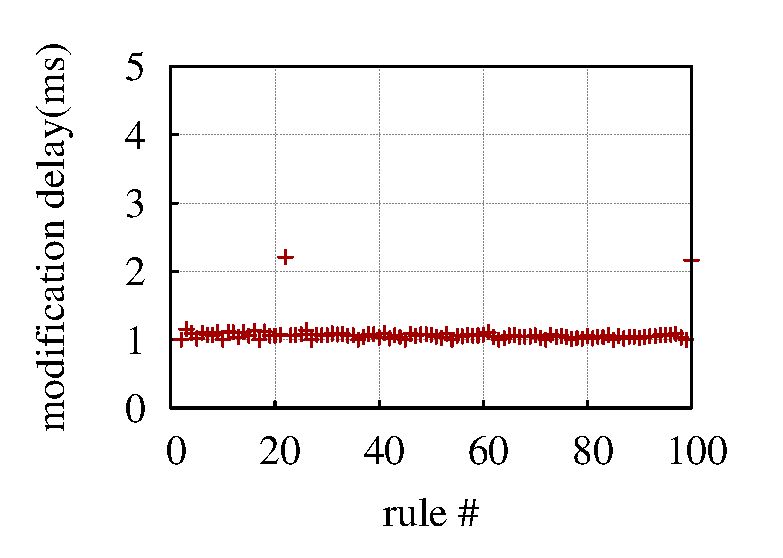
\includegraphics[width=.5\linewidth]{./figs/jan27_intel_mod_decr_burst_100.eps}}\hfill
%\subfloat[burst size 200, same priority.\label{fig:intel_mod_same_burst_200}]
%  {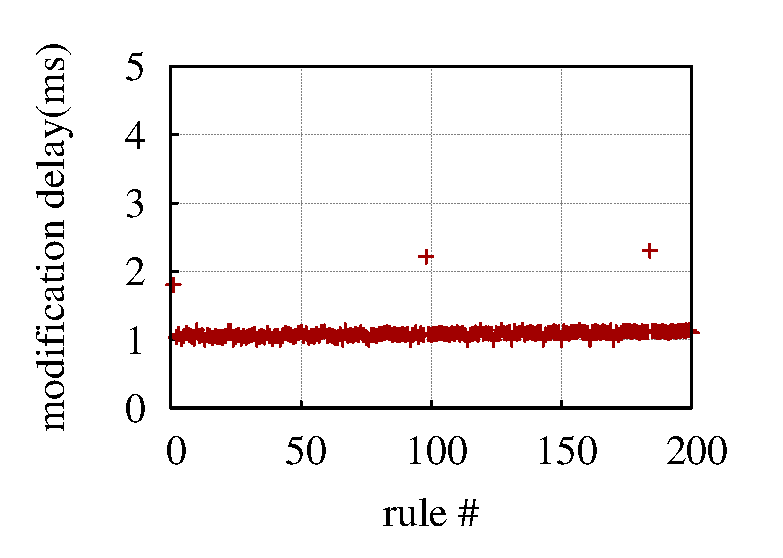
\includegraphics[width=.5\linewidth]{./figs/jan27_intel_mod_same_burst_200.eps}}
\caption{{\bf Intel} priority per-rule {\bf modification} latency results}
\label{fig:priority-intel-modify}
\end{figure}
\fi

%{\em Intel increasing/decreasing priority.} 
%Figure~\ref{fig:priority-intel-modify} shows the result for $B=100$ on
%Intel.
% , similar to insertion delay without
% priority.  We also tried other B values and the results are similar (omitted for brevity).


\minisection{Summary and root causes}
%Given our table occupancy and rule priority results, 
We conclude that the per-rule modification latency on \BroadcomOne and \IBM is 
impacted purely by table occupancy, not by rule priority structure.
For \BroadcomThree and \Intel, the per-rule modification delay 
%is 1 ms respectively 
is independent of rule priority, table occupancy, and burst size;
\BroadcomThree's per-rule modification delay is 2X higher than insertion.
%For \BroadcomThree, the modification delay is independent of rule priority but 
%is highly variable and is          
%related with table occupancy. The root cause of the variable and larger modification delay on 
%\BroadcomOne and \BroadcomThree is that modification involves insertion and deletion operation and it causes
%TCAM reorganization.

%We observe that flow rule priority do
%not impact modification delay. Modification delay in \BroadcomOne and \BroadcomThree is a
%function of table occupancy, whereas this is not the case for Intel where modification is as fast as insertion. 
Conversations with Broadcom indicated that TCAM modification should ideally be fast and independent of table size, 
so the underlying cause appears to be less optimized switch software in \BroadcomOne. Indeed, our measurements with \BroadcomThree show that this issue has (at least partly) been fixed.

% However, for Broadcom, the modification delay is much higher
% than rule insertion delay with same priority. For Intel, the modification delay
% is similar to rule insertion delay with same priority. 

% \aditya{missing causes!}


% LocalWords:  pre Broadcom

\subsubsection{Deletion Latency}
We now estimate the impact of rule deletions.
We use bursts of operations as before.
Denote
$T(r_i)$ as the first time we stopped observing packets matching rule $r_i$
from the intended port of the rule action. We define deletion latency
as $T(r_i)-T(r_{i-1})$.

\begin{figure}[!tb]
\centering
\subfloat[100 rules in table \label{fig:bcm_del_same_burst_100}]
  {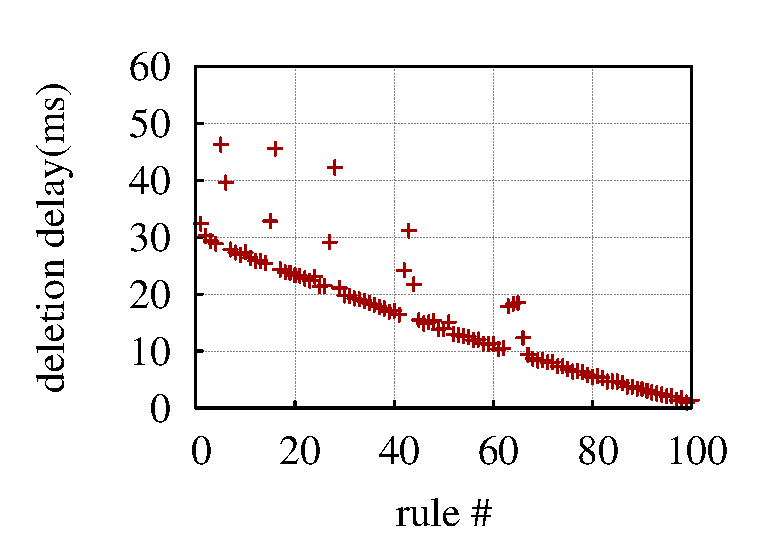
\includegraphics[width=.50\linewidth]{./figs/jan27_bcm_del_same_burst_100.eps}}\hfill
%\subfloat[burst size 100, increasing priority.\label{fig:bcm_del_incr_burst_100}]
%  {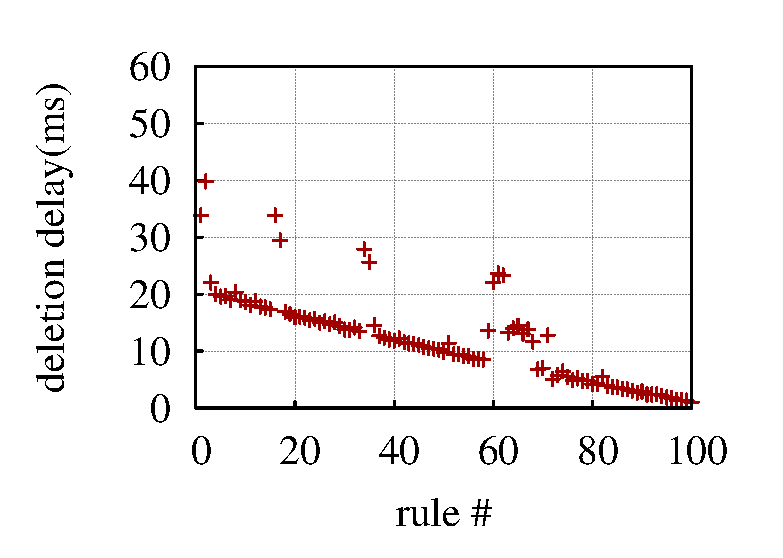
\includegraphics[width=.30\linewidth]{./figs/jan27_bcm_del_incr_burst_100.eps}}\hfill
\subfloat[200 rules in table \label{fig:bcm_del_same_burst_200}]
  {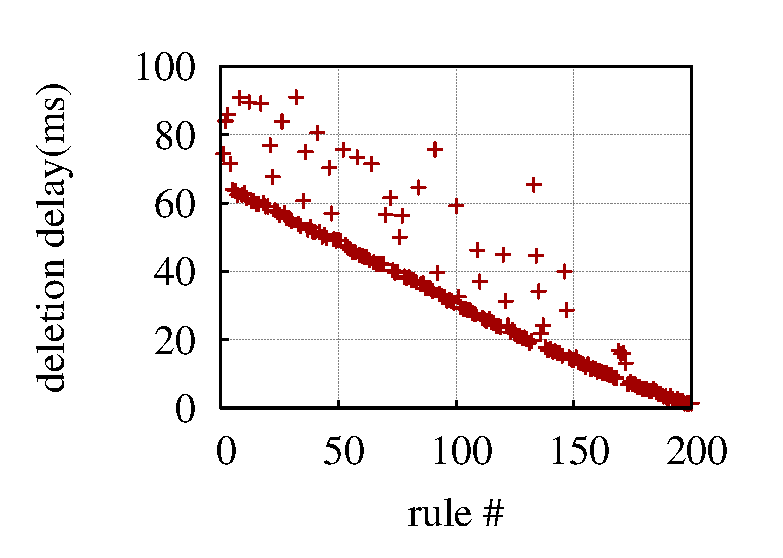
\includegraphics[width=.50\linewidth] {./figs/jan27_bcm_del_same_burst_200.eps}}
\compactcaption{ {\bf \BroadcomOne} per-rule {\bf del.} latency, same priority}
\label{fig:occupancy-broadcom-deletion}
\end{figure}

\begin{figure}[!tb]
\centering
\subfloat[100 rules in table\label{fig:intel_del_same_burst_100}]
  {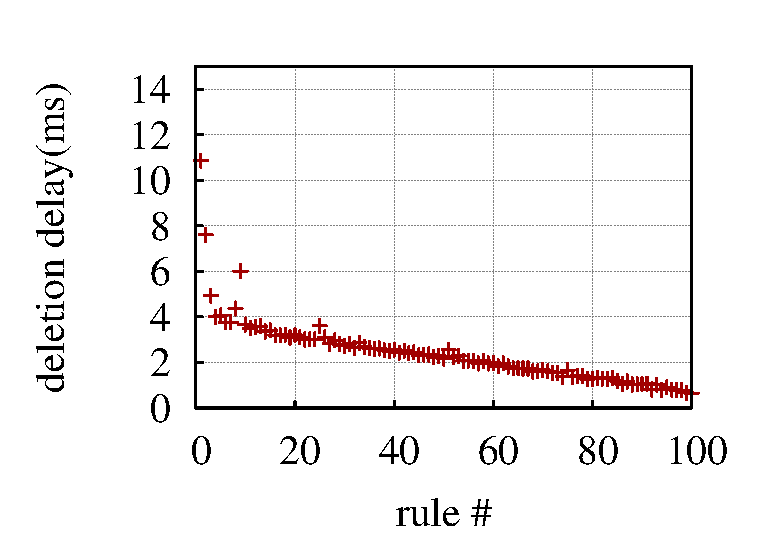
\includegraphics[width=.50\linewidth]{./figs/jan27_intel_del_same_burst_100.eps}}\hfill
%\subfloat[burst size 100, increasing priority.\label{fig:intel_del_incr_burst_100}]
%  {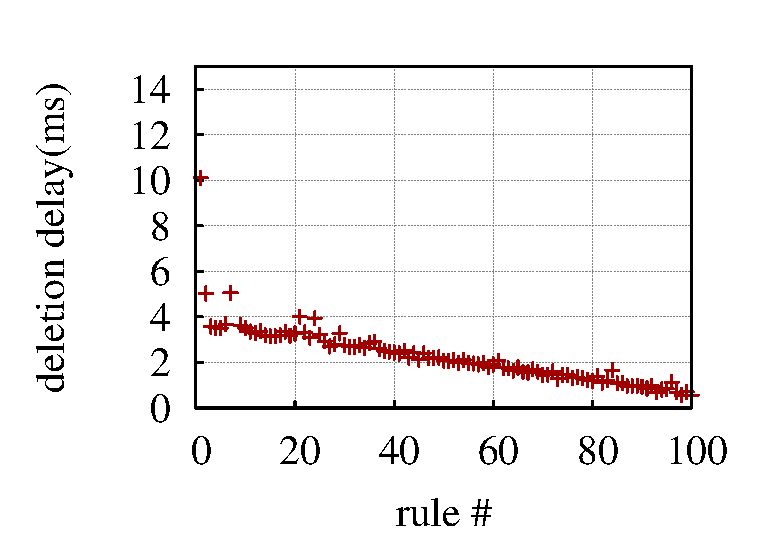
\includegraphics[width=.30\linewidth]{./figs/jan27_intel_del_incr_burst_100.eps}}\hfill
\subfloat[200 rules in table \label{fig:intel_del_same_burst_200}]
  {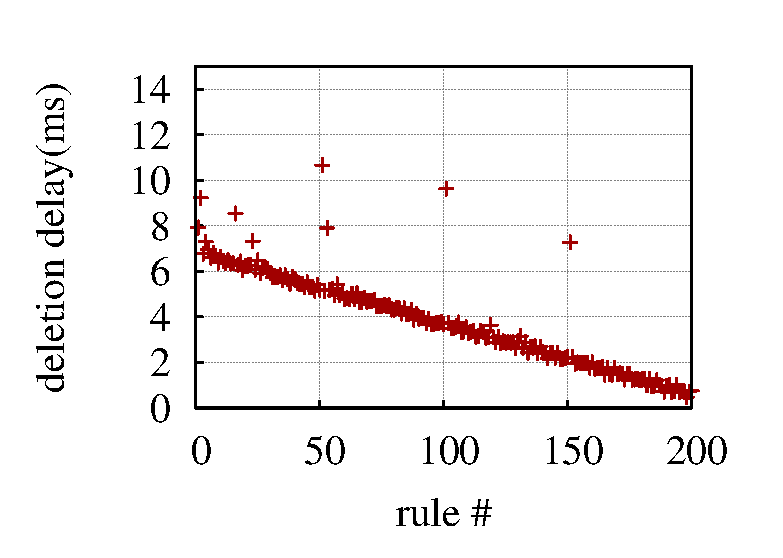
\includegraphics[width=.50\linewidth]{./figs/jan27_intel_same_burst_200.eps}}
\compactcaption{{\bf \Intel} per-rule {\bf del.} latency, same priority}
\label{fig:occupancy-intel-deletion}
\end{figure}

\minisection{Table Occupancy} We pre-insert $S$ rules into a switch, all with
the same priority. We then delete one rule at a time, sending deletion
requests back-to-back. The results for \BroadcomOne at $S=100$ and $S=200$
are shown in \figsref{fig:bcm_del_same_burst_100}{fig:bcm_del_same_burst_200},
respectively. We see that per rule deletion delay decreases as the table occupancy drops. We see a similar trend for Intel (\figsref{fig:intel_del_same_burst_100}{fig:intel_del_same_burst_200}) and \BroadcomThree (figure not shown).

%  and
% ~\ref{fig:occupancy-intel-deletion}, the per rule deletion delay
% decreases as the table occupancy drops.


\begin{figure}[!tb]
\centering
% \subfloat[burst size 100, same priority.\label{fig:bcm_del_same_burst_100}]
%   {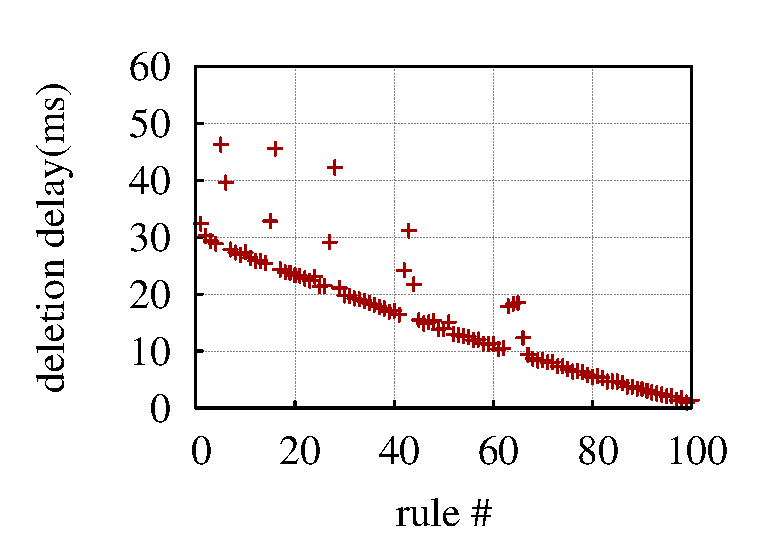
\includegraphics[width=.30\linewidth]{./figs/jan27_bcm_del_same_burst_100.eps}}\hfill
\subfloat[increasing priority\label{fig:bcm_del_incr_burst_100}]
  {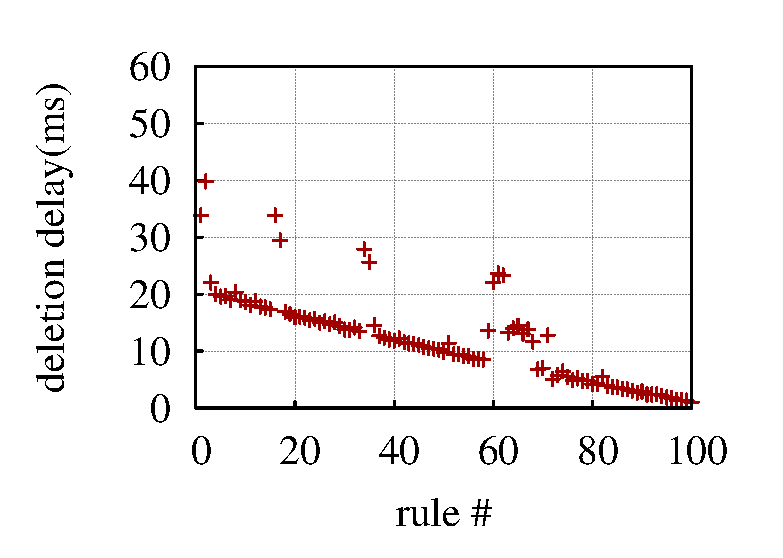
\includegraphics[width=.50\linewidth]{./figs/jan27_bcm_del_incr_burst_100.eps}}\hfill
\subfloat[decreasing priority\label{fig:bcm_del_decr_burst_100}]
  {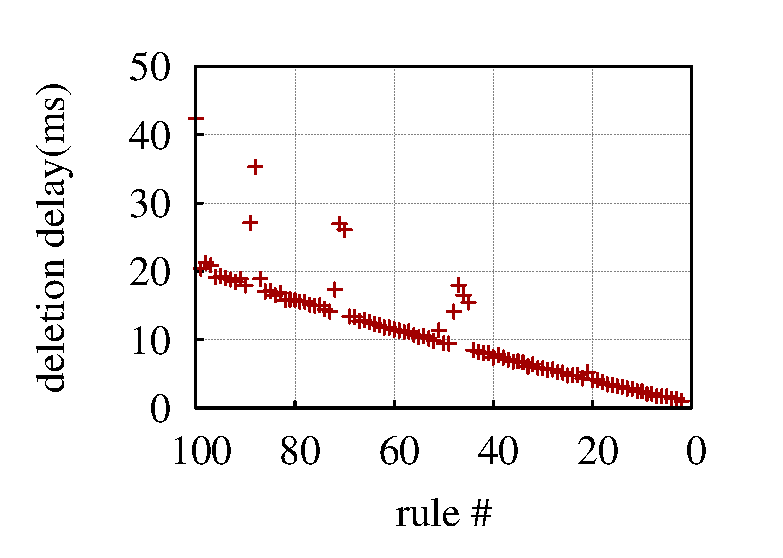
\includegraphics[width=.50\linewidth]{./figs/jan27_bcm_del_decr_burst_100.eps}}
\compactcaption{{\bf \BroadcomOne} priority per-rule {\bf del.} latency, 
    B=100}
\label{fig:priority-broadcom-deletion}
\end{figure}

\begin{figure}[!tb]
\centering
%\subfloat[burst size 100, same priority.\label{fig:jan27_intel_del_same_burst_100}]
%  {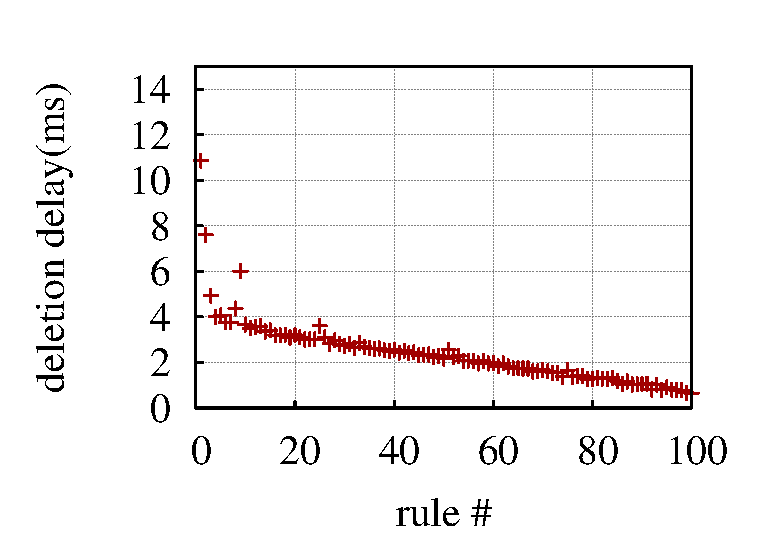
\includegraphics[width=.24\linewidth]{./figs/jan27_intel_del_same_burst_100.eps}}\hfill
%\subfloat[burst size 100, increasing priority.\label{fig:jan27_intel_del_incr_burst_100}]
%  {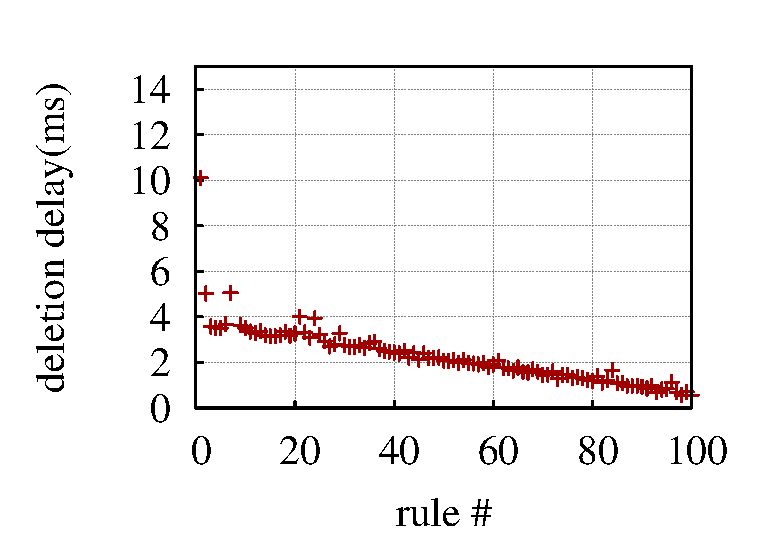
\includegraphics[width=.24\linewidth]{./figs/jan27_intel_del_incr_burst_100.eps}}\hfill
%\subfloat[burst size 100, decreasing priority.\label{fig:jan27_intel_del_decr_burst_100}]
%  {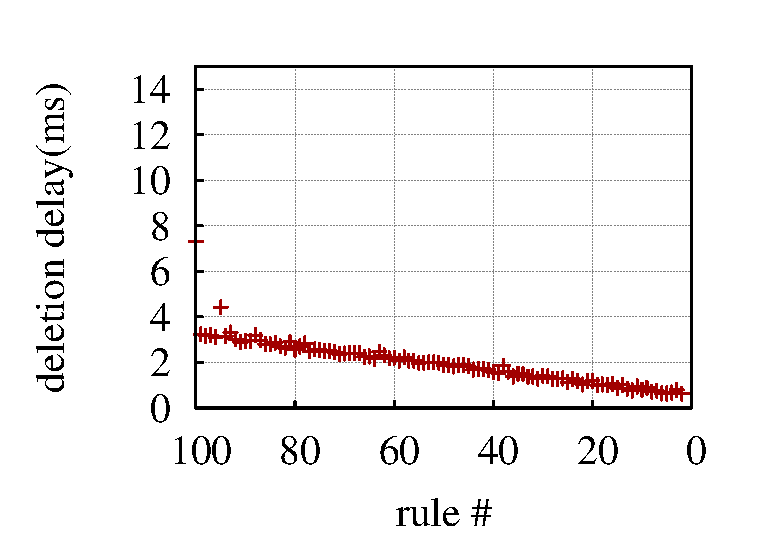
\includegraphics[width=.24\linewidth]{./figs/jan27_intel_del_decr_burst_100.eps}

% \subfloat[burst size 100, same priority.\label{fig:intel_intel_del_same_burst_100}]
%   {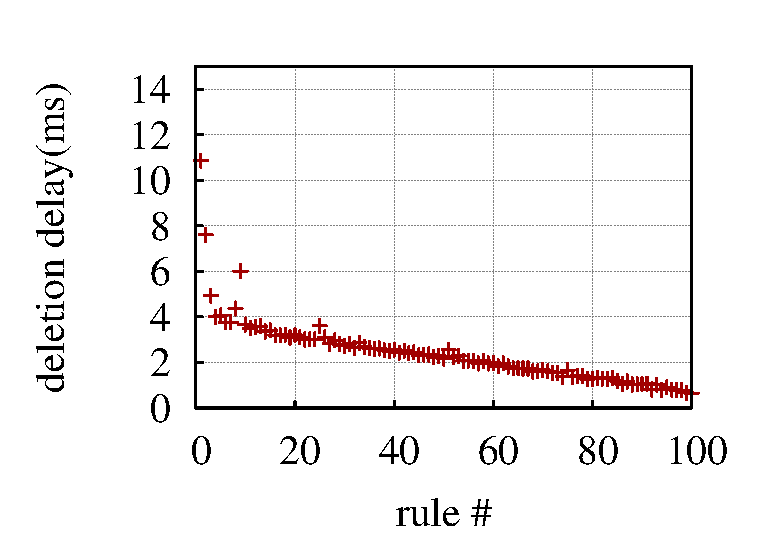
\includegraphics[width=.30\linewidth]{./figs/jan27_intel_del_same_burst_100.eps}}\hfill
\subfloat[increasing priority\label{fig:intel_del_incr_burst_100}]
  {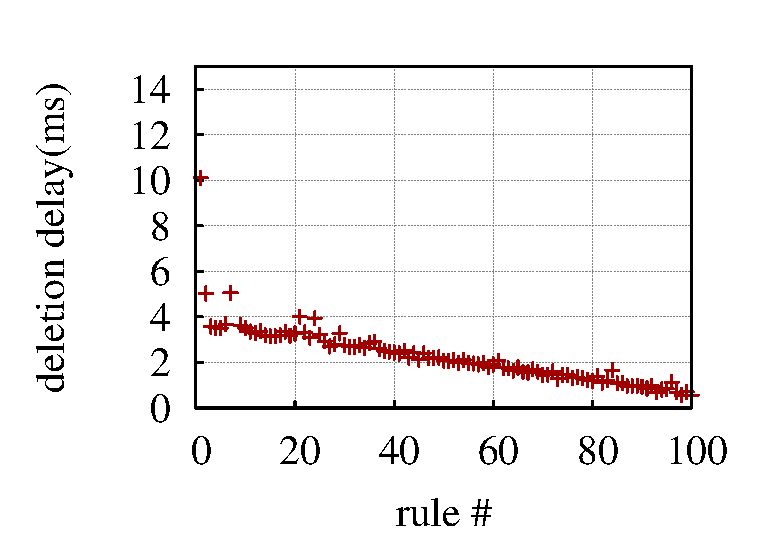
\includegraphics[width=.50\linewidth]{./figs/jan27_intel_del_incr_burst_100.eps}}\hfill
\subfloat[decreasing priority\label{fig:intel_del_decr_burst_100}]
  {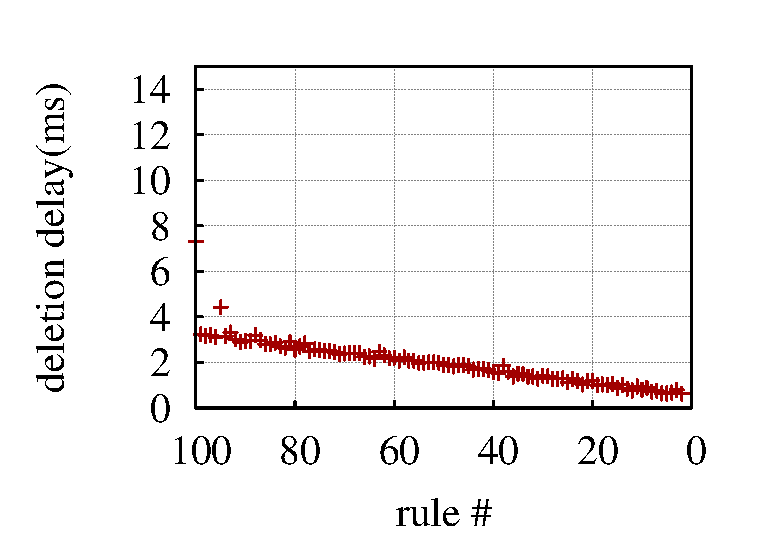
\includegraphics[width=.50\linewidth]{./figs/jan27_intel_del_decr_burst_100.eps}}

\compactcaption{{\bf Intel} priority per-rule {\bf del.} latency, B=100}
\label{fig:priority-intel-deletion}
\end{figure}


\minisection{Rule Priorities} We start with $B$ existing rules in the switch, 
and delete one rule at a time
%,``with'' and ``without priority''. In the former case, 
%we delete rules 
in increasing and decreasing priority order. 
For \BroadcomOne (\figref{fig:priority-broadcom-deletion}), \BroadcomThree
(figure not shown) and Intel (\figref{fig:priority-intel-deletion}), deletion 
is not affected by the priorities of rules in the table or the order of
deletion. %\aaron{Where are the without priority results?}


\minisection{\bf Root cause} Since deletion delay decreases with rule number 
in all cases, we conclude that deletion is incurring TCAM reordering.
% We observe that rule priority pattern does not affect deletion delay for both
% Broadcom and Intel. However, flow table occupancy affects deletion delay
% significant. Deletion delay can be much higher than insertion delay with same
% priority. 
% This seems to indicate that deletion incurs TCAM reordering in all
% cases in both switch architectures.
We also observe that processing rule timeouts at the switch does not
noticeably impact \flowmod operations. Given these two observations, we
recommend allowing rules to time out rather than explicitly deleting them, if
possible.

% LocalWords:  pre Broadcom TODO butbound TCAM

%\subsubsection{Impact of concurrent switch CPU jobs} 
\begin{figure}
\subfloat[init. table occupancy 0\label{fig:bcm_polling_table0_burst100}]
  {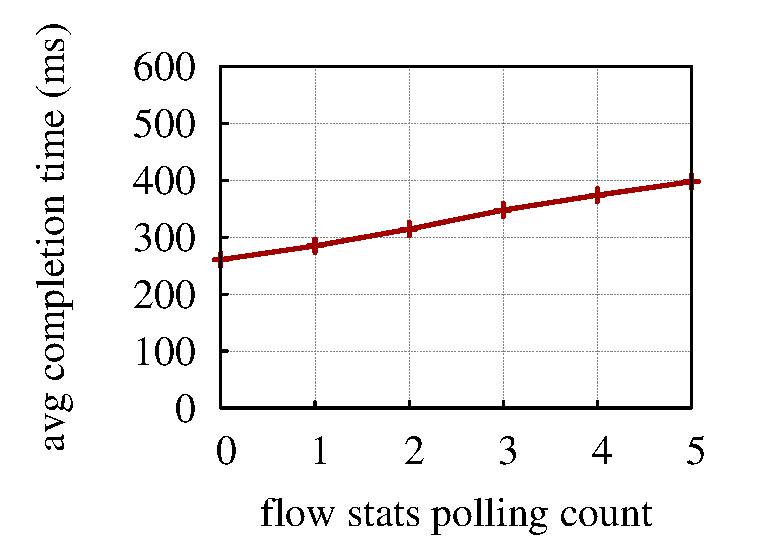
\includegraphics[width=0.25\textwidth]{./figs/bcm_polling_table0_burst100.eps}}
\subfloat[init. table occupancy 500\label{fig:bcm_polling_table500_burst100}]
  {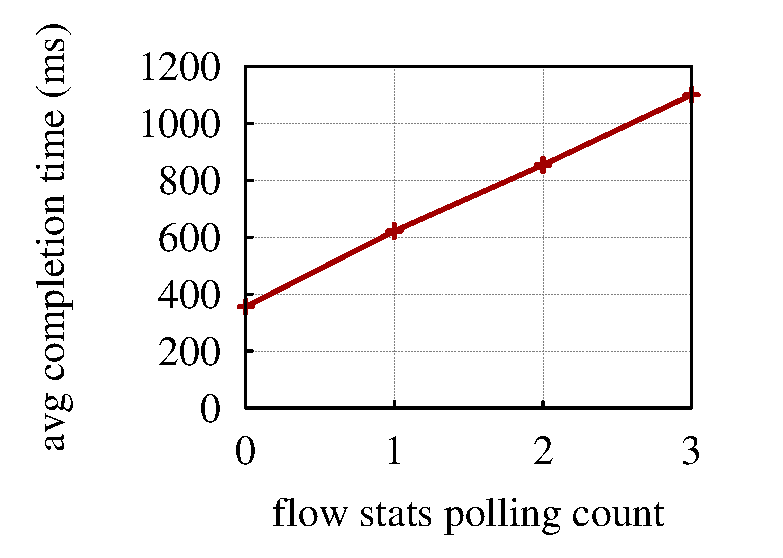
\includegraphics[width=0.25\textwidth]{./figs/bcm_polling_table500_burst100.eps}}\hfill
%\subfloat[controlled-rate mode, rate 50, polling frequency = 1/s\label{fig:bcm_polling_control_50_50_per_polling}]
%  {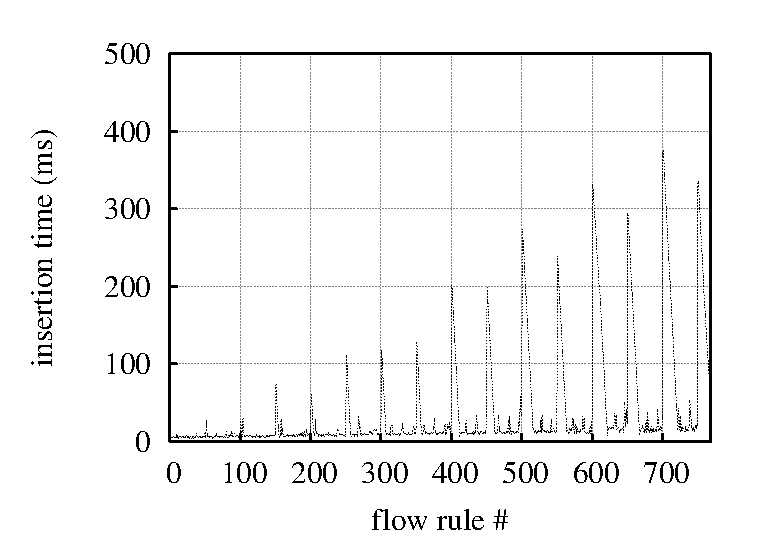
\includegraphics[width=0.3\textwidth]{./figs/bcm_polling_control_50_50_per_polling.eps}}
\topcompactcaption{Impact of polling on {\bf \BroadcomOne}, B=100}
%    ., simple rules (i.e., only specify destination IP)}
%\caption{{\bf Broadcom} per-rule {\bf insert} latency: impact of polling}
\label{fig:polling}
\end{figure}

We previously showed the impact of \flowmod processing on inbound latency
(\secref{s:measure_inbound}). We now study the impact of statistics
polling on outbound latency. 
%In particular,
%To investigate the impact of concurrent switch CPU activities, 
%we instruct the switch to report flow statistics.
%perform flow statistics queries. 
Figure~\ref{fig:polling} shows that concurrent activities, such as polling
statistics, can have a big impact on insertion delay, especially when table
occupancy is high: e.g., with \BroadcomOne, the total time to insert a 
burst of 100 same priority rules into a table with 500 rules is 853ms when 
two polling events occur during the insertion process, compared to
356ms without polling events.
%If we do not poll, the completion
%time of a burst insertion of 100 rules is 280 (xx) ms. If we poll all rules including
%recently installed 10 times during the burst insertion, the
%completion time becomes 490 (xx) ms. 
%\aditya{isn't this polling rate too high?} \aditya{what is the xx supposed to be?}
%$\li{Are we polling existing rule stats? It seems we also poll newly inserted
%  rule stats. What is polling count? }.
\iffalse
\subsection{Overall burst insertion completion time}
With the understanding of per-rule insertion latency, we present burst rule insertion
completion time as this is the metric many applications such as failover depend
on. 

\begin{figure}
\subfloat[insert low priority rules into\newline a table with high priority rules\label{fig:bcm_outbound_two_pri_high_low_burstB}]
  {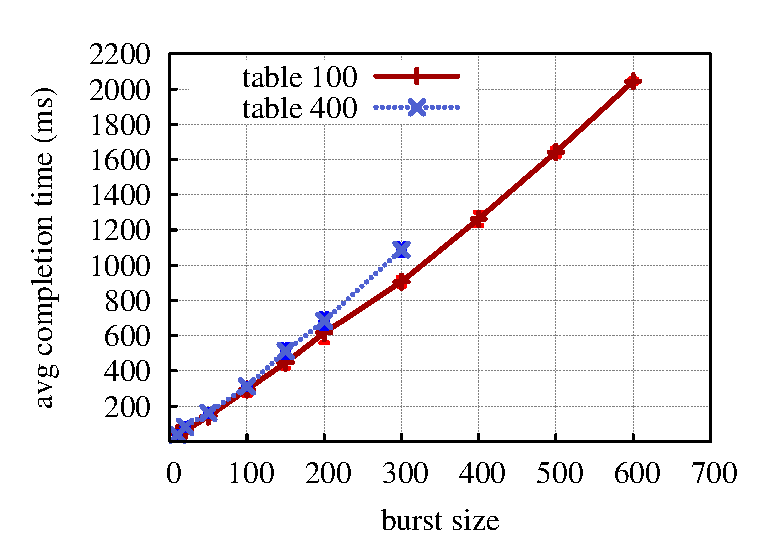
\includegraphics[width=.50\linewidth]{./figs/bcm_two_pri_high_low_burstB.eps}}\hfill
\subfloat[insert high priority rules into a table with low priority rules\label{fig:bcm_outbound_two_pri_low_high_burstB}]
  {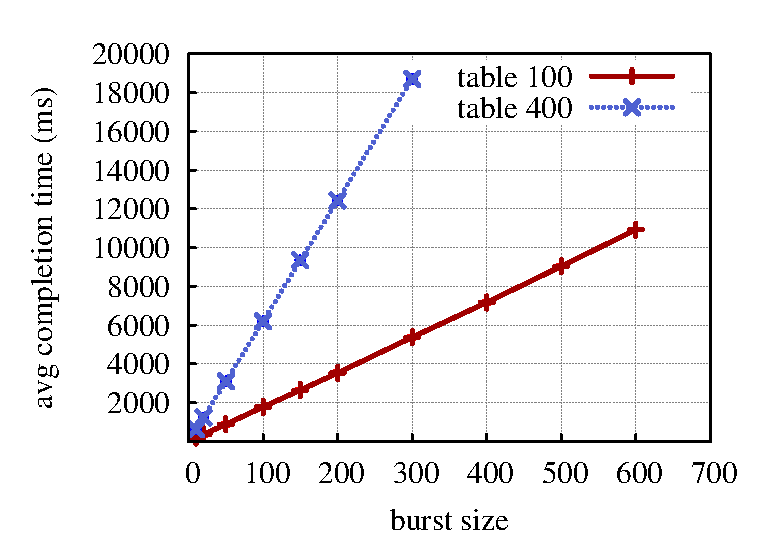
\includegraphics[width=.50\linewidth]{./figs/bcm_two_pri_low_high_burstB.eps}}
\compactcaption{Overall completion time on {\bf \BroadcomOne}.  Initial table
occupancy is S high (low) priority rules; insert a burst of low (high)
priority rules. Averaged over 5 runs. }
\label{fig:burst-completion-time}
\end{figure}
\fi




\iffalse
\begin{figure}[!tb]
\centering
%\subfloat[burst size 100, same priority.\label{fig:intel_burst_100_same_pri}]
%  {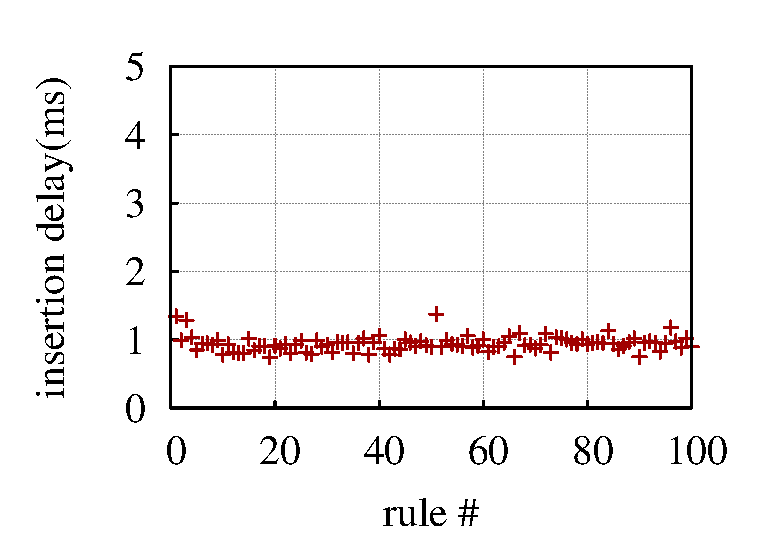
\includegraphics[width=.24\linewidth]{./figs/jan27_intel_same_burst_100.eps}}\hfill
%\subfloat[burst size 200, same priority.\label{fig:intel_burst_200_same_pri}]
%  {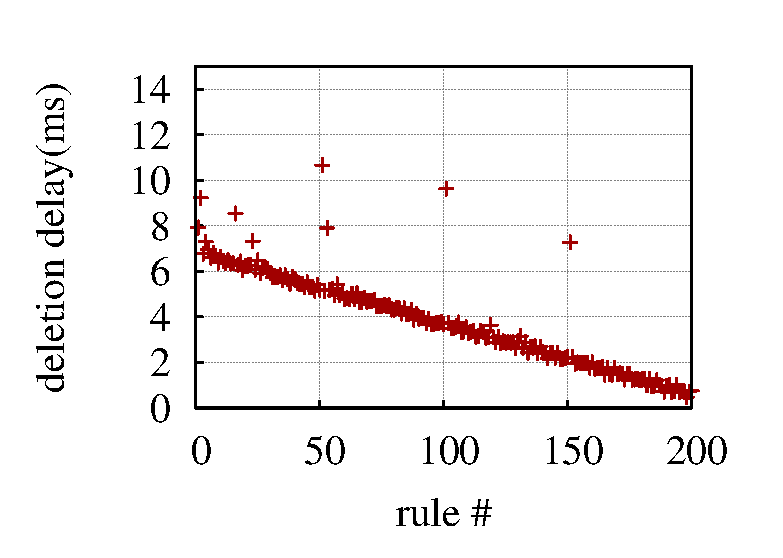
\includegraphics[width=.24\linewidth]{./figs/jan27_intel_same_burst_200.eps}}\hfill
%\subfloat[burst size 800 of low priority, table has 3200 high priority rules\label{fig:intel_burst_200_same_pri}]
%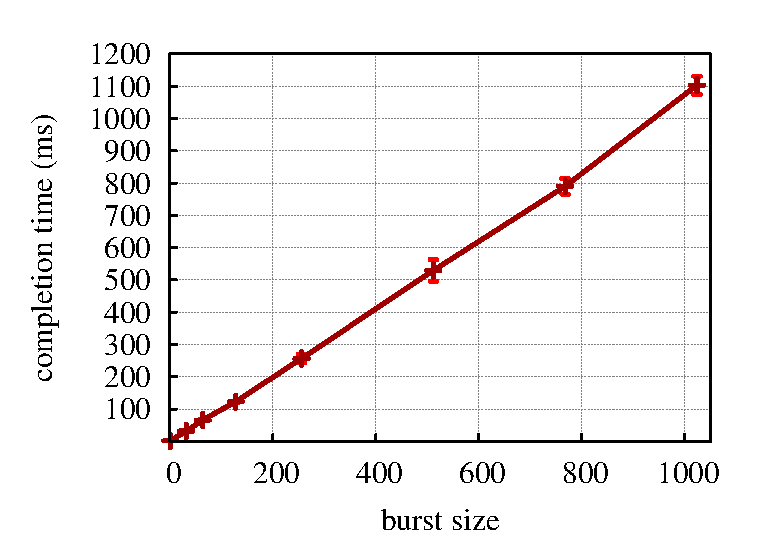
\epsfig{file=./figs/Intel_burst_effect_same.eps,width=0.5\textwidth}
%  {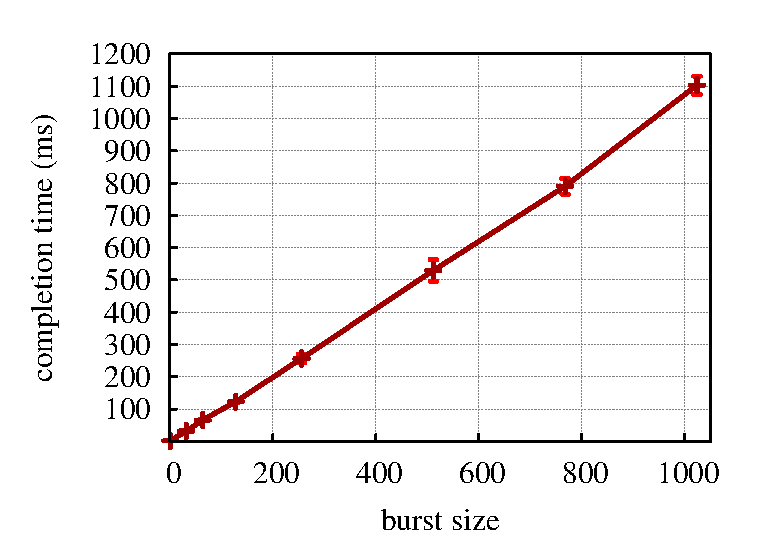
\includegraphics[width=.5\linewidth]{./figs/jan27_intel_burst_effect_same.eps}}\hfill %jan27_intel_decr_burst_100.eps
%   {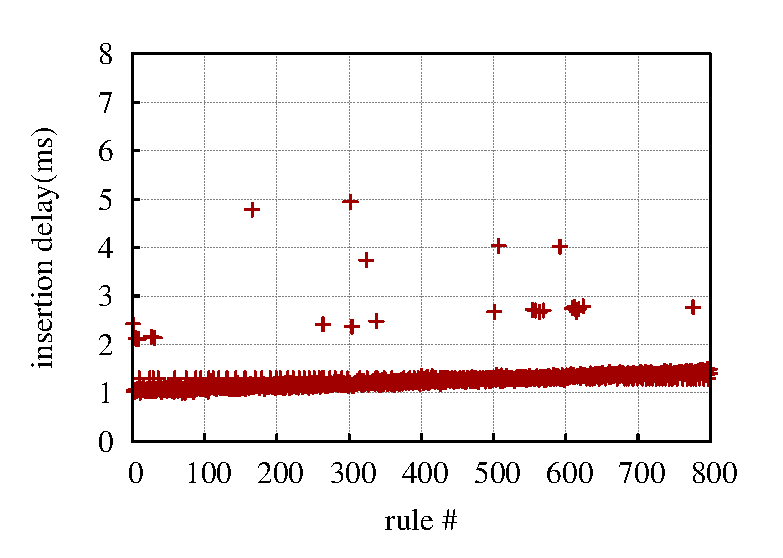
\includegraphics[width=.5\linewidth]{./figs/jan27_intel_3200H_800L_L_to_H_delta.eps}} \hfill
\subfloat[decreasing priority\label{fig:intel_burst_100_incr_pri_1}]
  {\includegraphics[width=.7\linewidth]{./figs/jan27_intel_decr_burst_size_effect.eps}}\hfill %jan27_intel_decr_burst_100.eps
%\subfloat[burst size 200, decreasing priority.\label{fig:intel_burst_200_incr_pri}]
%  {\includegraphics[width=.5\linewidth]{figs/jan27_intel_3200H_800L_decr.eps}}
%\subfloat[burst size 200, decreasing priority.\label{fig:intel_burst_200_decr_pri}]
%  {\includegraphics[width=.24\linewidth]{figs/jan27_intel_decr_burst_size_effect.eps}
\caption{{\bf Intel} overall completion time} 
\label{fig:priority-intel-insert-more-results}
\end{figure}
\fi
%\aditya{Is figure 14a correct? It says same priority}
\iffalse
We conduct two experiments. With $S$ rules in the table, we insert a burst of $B$ rules. 
For the first experiment, $S$ has high priority and we insert the burst with low priority. 
For the second experiment, if it is Broadcom (\BroadcomOne or \BroadcomThree), $S$ has low priority and we insert rules with high priority; 
if it is Intel, $S$ has high priority and we insert rules in {\em decreasing} priority.

For Broadcom, based on our hypothesis, as long as the same number of
rules get displaced, the completion time should be the same. Indeed,
 from \figref{fig:bcm_outbound_two_pri_high_low_burstB} (for \BroadcomOne), we see that even with
400 high priority rules in the table, the insertion delay for the
first experiment is no different from the setting when there is only
100 high priority rules in the table. In
\figref{fig:bcm_outbound_two_pri_low_high_burstB}, since newly inserted high
priority rules will displace 400 low priority rules in the table, the
completion time will be about three times higher than $S=100$.
 % If we
% insert in increasing priority, because each rule displaces different
% number of rules (rule $i$ displaces $i-1$ previous inserted rules),
% the total rule displacement is quadratic. Thus, the completion time
% will be quadratic with respect to burst sizes in this case (not
% shown).
%We clearly see this effect in
%Figure~\ref{fig:burst-completion-time-inc}.   
%\li{TODO: Do we need corresponding  results from Intel?} 


%\aditya{the rest does not make full sense. what is ``the first experiment''}

For Intel, % if $S$ has low priority and we insert rules with high priority, then
% it is the same as the first experiment.
we also run the same two experiments as for Broadcom. The results are similar to rule
insertion with same priority. This indicates that Intel optimizes for rule priority better
than Broadcom.  When we insert in decreasing
priority, 
%as shown in Figure~\ref{fig:priority-intel-insert-more-results}, 
the completion time is about 3.5 seconds, three times higher than the case of
insertion with same priority.
%the case in
%Figure~\ref{fig:priority-intel-insert-more-results}-a 
%where we insert a burst of
%800 low priority rules in a table with 3200 high priority rules installed.
%These results provide solid foundations for us to design solutions
%to tame latency in the subsequent sections.
\fi



% LocalWords:  init Broadcom openflow IP justs failover

